\chapter{QUIC}
\label{chap:quic}

O QUIC \citep{rfc8999, rfc9000} é um protocolo de transporte desenvolvido para reduzir a latência, melhorar a eficiência e aumentar a confiabilidade das comunicações na Internet. Diferentemente da pilha tradicional, que combina TCP e TLS em camadas separadas, o QUIC opera sobre o UDP, o que facilita sua implantação em redes existentes e sua implementação no espaço de usuário. Além disso, o QUIC integra o \textit{handshake} do TLS~1.3 ao seu próprio \textit{handshake} de transporte \citep{rfc9001}. Essa integração permite estabelecer uma conexão segura em um único RTT (\textit{Round-Trip Time}), ou em zero RTT na retomada de sessão, enquanto a combinação de TCP e TLS exige dois RTTs com TLS~1.3 ou três com TLS~1.2.

O QUIC também define seu próprio identificador de conexão, o \textit{Connection ID}. No TCP, uma conexão é identificada pela quádrupla formada pelos endereços IP e pelas portas de origem e destino, de modo que a alteração de qualquer um desses valores interrompe a conexão. O QUIC, por sua vez, identifica a conexão pelo \textit{Connection ID}, o que permite mantê-la ativa após uma mudança no caminho de rede, como na migração de um dispositivo de uma rede Wi-Fi para uma rede celular, sem a necessidade de restabelecê-la. Esse mecanismo é denominado \textit{Connection Migration}.

\section{Recursos do QUIC utilizados na proposta}

Na infraestrutura proposta, o QUIC é executado nos \textit{gateways} e transporta os dados das aplicações TCP locais por meio de \textit{streams}. O ICE realiza a descoberta e a seleção dos caminhos de comunicação. Assim, o estabelecimento da conexão QUIC constitui uma etapa do processo completo, que também envolve a sinalização e as verificações de conectividade.

A implementação permite o uso de 0-RTT e de migração de conexão, mas esses recursos não foram avaliados explicitamente nos experimentos. Sua utilização permanece condicionada à disponibilidade de caminhos de comunicação viabilizados pelo ICE, incluindo os mecanismos de travessia de NAT necessários. Portanto, os resultados apresentados não caracterizam os ganhos de latência do 0-RTT nem a continuidade da comunicação durante uma migração.

A abordagem adotada utiliza ICE para estabelecer o caminho de comunicação, em vez da variante de \textit{hole punching} baseada em migração de conexão discutida neste capítulo na Seção \ref{sec:quic_hole_punching}. Os detalhes da integração entre QUIC e ICE são apresentados no Capítulo~\ref{chap:implementation}.

\section{História do QUIC}

O desenvolvimento do QUIC foi motivado pelas limitações da pilha tradicional TCP/TLS/HTTP \citep{marx2020quic}, ilustrada na Figura~\ref{fig:tcp_http_stack}. Embora o HTTP/2 tenha introduzido a multiplexação de fluxos sobre uma única conexão, ele ainda depende do TCP, que entrega os bytes estritamente em ordem. Assim, a perda de um único segmento bloqueia a entrega dos dados de todos os fluxos multiplexados até a sua retransmissão, problema conhecido como \textit{Head-of-Line Blocking}. Além disso, \textit{middleboxes}, como NATs e \textit{firewalls}, inspecionam e, por vezes, modificam o cabeçalho TCP, descartando pacotes com opções desconhecidas, o que dificulta a evolução do protocolo. A implementação do TCP no núcleo do sistema operacional também retarda a adoção de novas funcionalidades. Por fim, mudanças de mapeamento de endereço realizadas pelos próprios NATs, como o \textit{NAT rebinding}, interrompem conexões TCP, pois estas são identificadas pela quádrupla de endereços e portas.

\begin{figure}[!ht]
    \centering
    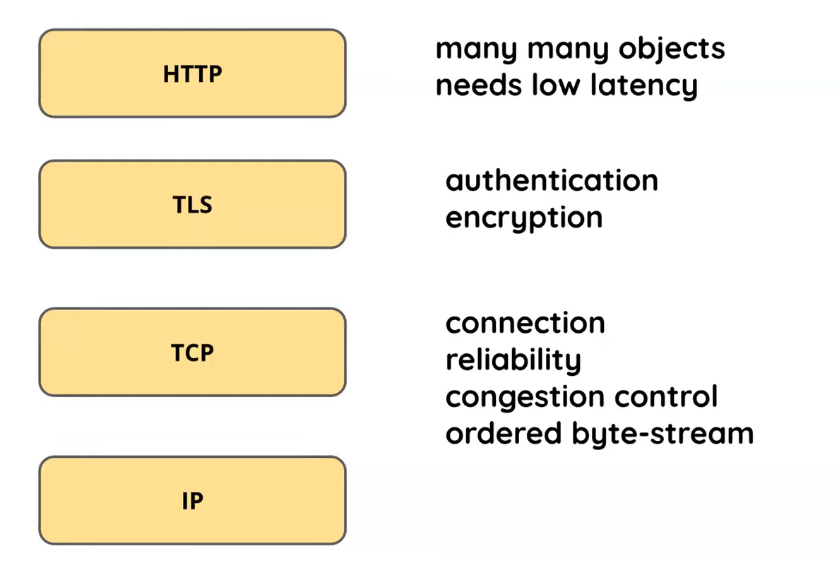
\includegraphics[width=0.7\textwidth]{fig/QUIC/tcp_http_stack.png}
    \caption{Pilha tradicional TCP/TLS/HTTP. Fonte: adaptado de \citep{marx2020quic}.}
    \label{fig:tcp_http_stack}
\end{figure}

A latência é um fator crítico para aplicações como \textit{streaming} de vídeo, navegação \textit{web} interativa e sistemas de tempo real, nas quais pequenas reduções no tempo de resposta melhoram a experiência do usuário. O QUIC foi projetado para superar as limitações descritas acima, oferecendo um protocolo de transporte mais flexível e com menor latência no estabelecimento de conexões.

Entre as principais características do QUIC, destacam-se:

\begin{itemize}
\item Integração com o TLS~1.3, que torna obrigatória a cifragem e a autenticação de todo o tráfego \citep{rfc9001};
\item Estabelecimento de conexão em 1-RTT e retomada de sessão em 0-RTT;
\item Múltiplos fluxos (\textit{streams}) independentes em uma mesma conexão, o que elimina o \textit{Head-of-Line Blocking} entre fluxos;
\item Detecção de perdas e controle de congestionamento implementados no espaço de usuário, com números de pacote monotonicamente crescentes que eliminam a ambiguidade nas retransmissões \citep{rfc9002};
\item Identificadores de conexão (\textit{Connection IDs}), que permitem a migração da conexão entre redes;
\item Proteção de cabeçalho, que cifra metadados como o número de pacote;
\item Suporte a protocolos de aplicação, como o HTTP/3, que exploram essas características.
\end{itemize}

\subsection{GQUIC (Google QUIC)}

O GQUIC foi a implementação original do QUIC, desenvolvida pelo Google a partir de 2012 com o objetivo de melhorar o desempenho do tráfego HTTPS \citep{marx2020quic}. Diferentemente da versão padronizada, o GQUIC utilizava um protocolo criptográfico próprio, o QUIC Crypto, em vez do TLS. Implantado de forma experimental nos serviços do Google, o GQUIC representava, em 2017, mais de 30\% do tráfego de saída da empresa, o que demonstrou na prática que um protocolo baseado em UDP com segurança integrada reduz a latência das conexões \textit{web}.

A arquitetura do GQUIC, ilustrada na Figura~\ref{fig:gquic_stack}, já incorporava conceitos posteriormente adotados pelo QUIC padronizado, como a multiplexação de fluxos, a criptografia integrada ao transporte e o estabelecimento de conexão com menos RTTs.

\begin{figure}[!ht]
    \centering
    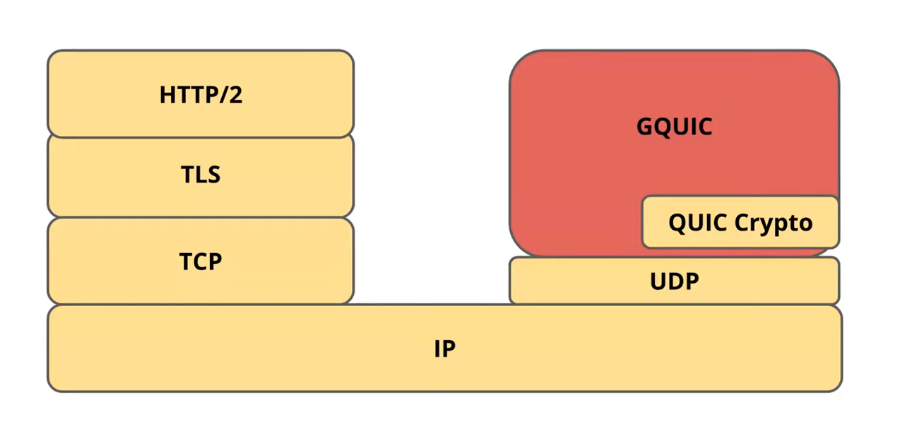
\includegraphics[width=0.7\textwidth]{fig/QUIC/gquic_stack.png}
    \caption{Arquitetura do GQUIC. Fonte: adaptado de \citep{marx2020quic}.}
    \label{fig:gquic_stack}
\end{figure}

\subsection{IQUIC (IETF QUIC)}

Em 2016, a IETF (\textit{Internet Engineering Task Force}) criou o grupo de trabalho QUIC, com o objetivo de padronizar o protocolo a partir da experiência obtida com o GQUIC. A versão resultante é denominada IETF QUIC, ou IQUIC. Durante a padronização, o protocolo recebeu diversas alterações, entre elas a substituição do QUIC Crypto pelo \textit{handshake} do TLS~1.3, novos formatos de cabeçalho, identificadores de conexão de tamanho variável escolhidos por cada \textit{endpoint}, a proteção do número de pacote e a definição de fluxos unidirecionais e bidirecionais. A padronização também separou o protocolo de transporte do mapeamento do HTTP, o que deu origem ao HTTP/3.

O resultado desse processo foi a primeira versão padronizada do protocolo, o QUICv1, publicada em 2021 \citep{rfc9000}, que serve de base para o HTTP/3. A Figura~\ref{fig:quic_stack} mostra a pilha de protocolos com o QUIC, na qual o protocolo de transporte incorpora funcionalidades antes distribuídas entre o TCP e o TLS.

\begin{figure}[!ht]
    \centering
    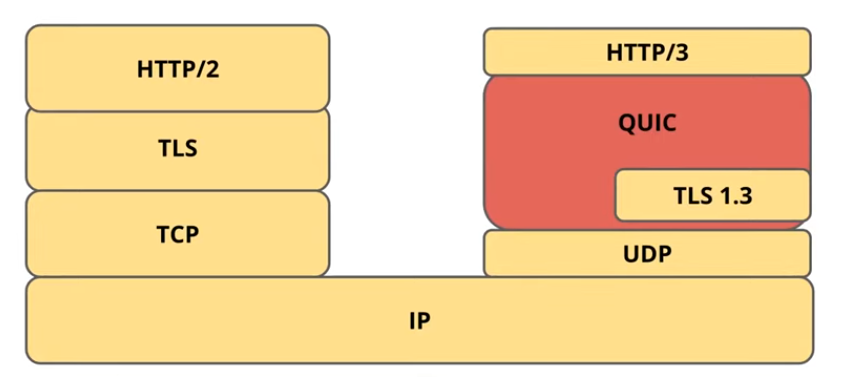
\includegraphics[width=0.7\textwidth]{fig/QUIC/quic_stack.png}
    \caption{Pilha de protocolos utilizando QUIC. Fonte: adaptado de \citep{marx2020quic}.}
    \label{fig:quic_stack}
\end{figure}

\section{Pacotes do QUIC}
\label{sec:quic_packets}

O QUIC define dois formatos de pacote \citep{rfc9000}: os pacotes com \textit{long header} e os pacotes com \textit{short header}. Cada pacote transporta um ou mais \textit{frames}, que são as unidades de informação do protocolo e podem conter dados de aplicação, como os \textit{frames} \texttt{STREAM}, ou informações de controle, como os \textit{frames} \texttt{ACK}. Os pacotes QUIC são transportados em datagramas UDP, e um mesmo datagrama pode conter vários pacotes QUIC, mecanismo denominado \textit{coalescing}. Como o \textit{short header} não possui campo de tamanho, um pacote com esse cabeçalho deve ser o último do datagrama. A Figura~\ref{fig:quic_encapsulation_packet} ilustra essa estrutura.

\begin{figure}[!ht]
    \centering
    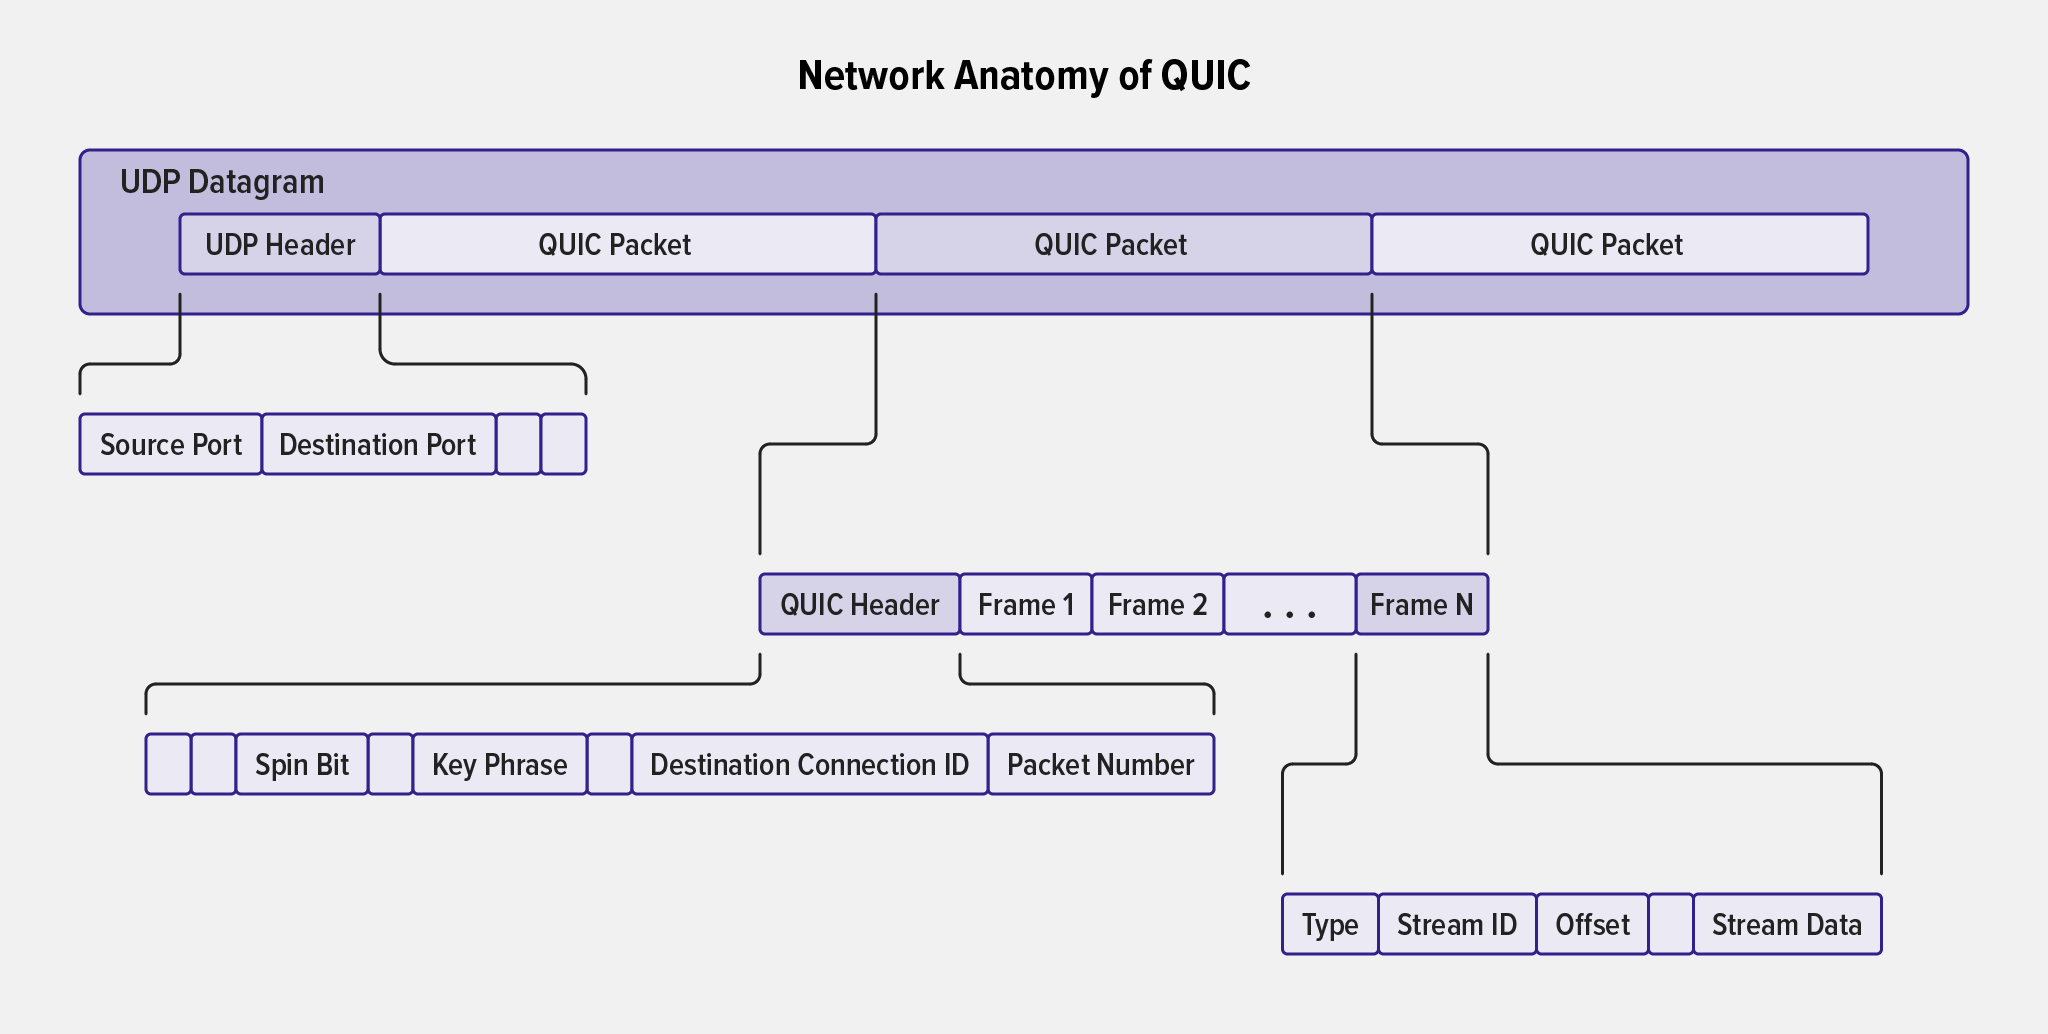
\includegraphics[width=0.9\textwidth]{fig/QUIC/quic_encapsulation_packet.png}
    \caption{Encapsulamento de pacotes QUIC em um datagrama UDP. Fonte: adaptado de \citep{f5_quic_http3}.}
    \label{fig:quic_encapsulation_packet}
\end{figure}


Cada formato de cabeçalho se subdivide em tipos de pacote, e cada tipo cumpre uma função em uma etapa específica da conexão. Os pacotes com \textit{long header} compreendem os tipos \texttt{Initial}, \texttt{0-RTT}, \texttt{Handshake} e \texttt{Retry}, utilizados durante o estabelecimento da conexão, enquanto o \textit{short header} possui um único tipo, o \texttt{1-RTT}, utilizado após o \textit{handshake}. Cada tipo de pacote pode transportar apenas determinados tipos de \textit{frame}, conforme a Tabela~\ref{tab:quic_frames_tab}.

Há ainda o pacote de \textit{Version Negotiation}, enviado pelo servidor quando este não suporta a versão proposta pelo cliente. Esse pacote utiliza o formato de \textit{long header}, com o campo de versão igual a zero, e não pertence a nenhuma versão específica do QUIC \citep{rfc8999}. A Seção~\ref{sec:version_negotiation_packet} descreve esse pacote.

\subsection{Cabeçalhos do QUIC}
\label{sec:quic_headers}

O RFC~8999 \citep{rfc8999} define as propriedades do QUIC independentes de versão, entre elas os dois formatos de cabeçalho: o \textit{long header} e o \textit{short header}. O primeiro é utilizado durante o estabelecimento da conexão, enquanto o segundo é utilizado a partir do momento em que as chaves 1-RTT estão disponíveis. Os demais campos de cada formato dependem da versão do protocolo. Este trabalho adota a primeira versão, o QUICv1, e descreve os campos conforme o RFC~9000 \citep{rfc9000}.

\subsubsection{Long Header}
\label{sec:quic_long_header}

\begin{figure}[!ht]
        \centering
        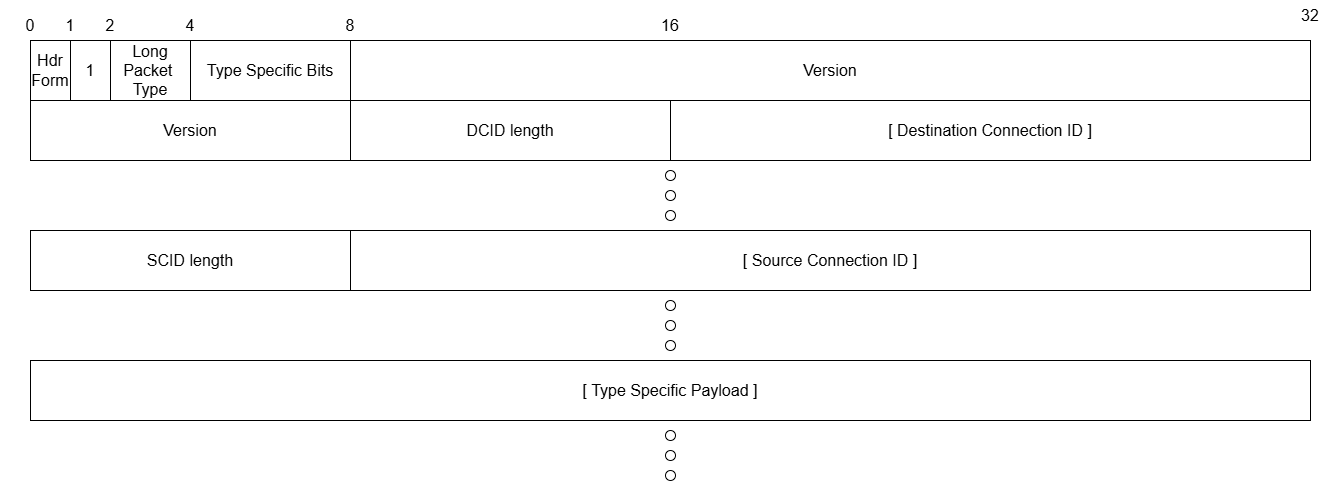
\includegraphics[width=1.0\linewidth]{fig/QUIC/quic_long_header.png}
        \caption{Cabeçalho longo do QUIC.}
        \label{fig:quic_long_header}
\end{figure}

A Figura~\ref{fig:quic_long_header} apresenta o formato do \textit{long header}, utilizado pelos quatro tipos de pacote listados na Tabela~\ref{tab:quic_long_header_packets} e descritos na Seção~\ref{sec:quic_long_header_packets}. O RFC~9000 \citep{rfc9000} define os campos comuns a esses pacotes e os campos específicos de cada tipo, descritos a seguir:


\begin{table}[!ht]
    \centering
    \setstretch{1.3}
    \begin{tabular}{|c|c|}
        \hline
        \textbf{Valor} & \textbf{Tipo de pacote} \\
        \hline
        0x00 & Initial   \\
        0x01 & 0-RTT     \\
        0x02 & Handshake \\
        0x03 & Retry     \\
        \hline
    \end{tabular}
    \caption{Tipos de pacotes QUIC com \textit{long header}. Fonte: \citep{rfc9000}.}
    \label{tab:quic_long_header_packets}
\end{table}

\begin{itemize}
    \item \textbf{Primeiro byte:}
    \begin{itemize}
        \item \textbf{Header Form} (1 bit): identifica o formato do cabeçalho; no \textit{long header}, possui sempre o valor 1;
        \item \textbf{Fixed Bit} (1 bit): possui sempre o valor 1, exceto em pacotes de \textit{Version Negotiation};
        \item \textbf{Long Packet Type} (2 bits): identifica o tipo de pacote, conforme a Tabela~\ref{tab:quic_long_header_packets};
        \item \textbf{Type-Specific Bits} (4 bits): bits cujo significado depende do tipo de pacote. Nos pacotes \texttt{Initial}, \texttt{0-RTT} e \texttt{Handshake}, esses bits contêm dois bits reservados e o campo \textit{Packet Number Length};
    \end{itemize}
    \item \textbf{Version} (32 bits): identifica a versão do QUIC e determina a interpretação dos demais campos; no QUICv1, possui o valor \texttt{0x00000001};
    \item \textbf{Destination Connection ID Length} (8 bits): indica o tamanho, em bytes, do campo seguinte;
    \item \textbf{Destination Connection ID} (DCID, 0 a 160 bits): identificador de conexão escolhido pelo receptor do pacote;
    \item \textbf{Source Connection ID Length} (8 bits): indica o tamanho, em bytes, do campo seguinte;
    \item \textbf{Source Connection ID} (SCID, 0 a 160 bits): identificador de conexão escolhido pelo emissor do pacote;
    \item \textbf{Type-Specific Payload}: campos específicos de cada tipo de pacote, descritos na Seção~\ref{sec:quic_long_header_packets}.
\end{itemize}

\subsubsection{Short Header}
\label{sec:quic_short_header}



A Figura~\ref{fig:quic_short_header} apresenta o formato do \textit{short header}. Diferentemente do \textit{long header}, que transporta informações necessárias apenas ao estabelecimento da conexão, como a versão e os comprimentos dos \textit{Connection IDs}, o \textit{short header} é utilizado na transmissão de dados e de controle ao longo da conexão e, por isso, é mais compacto. Pacotes com \textit{short header} podem ser enviados antes do término do \textit{handshake}, assim que as chaves 1-RTT estão disponíveis; no caso do servidor, isso ocorre logo após o envio de sua mensagem \texttt{Finished}.

\begin{figure}[!ht]
        \centering
        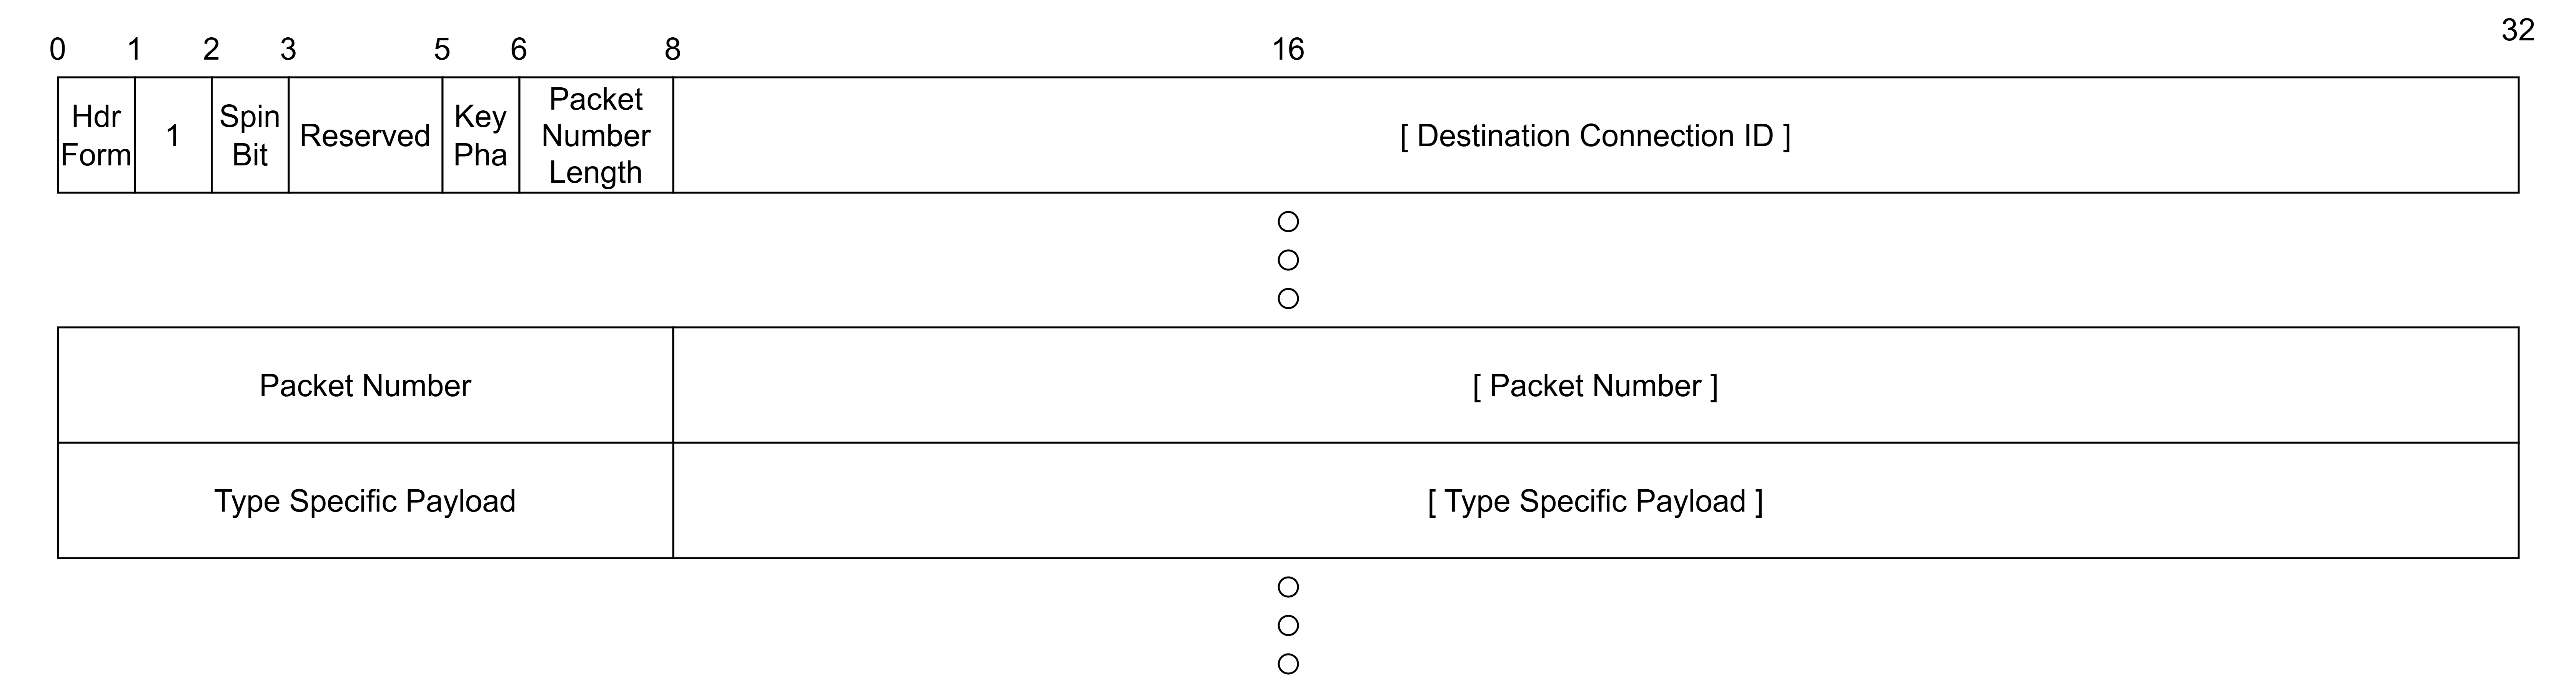
\includegraphics[width=1.0\linewidth]{fig/QUIC/quic_short_header.png}
        \caption{Cabeçalho curto do QUIC.}
        \label{fig:quic_short_header}
\end{figure}


O \textit{short header} possui um único tipo de pacote, o \texttt{1-RTT}, descrito na Seção~\ref{sec:quic_short_header_packets}. O RFC~9000 \citep{rfc9000} define seus campos, descritos a seguir:

\begin{itemize}
    \item \textbf{Primeiro byte:}
    \begin{itemize}
        \item \textbf{Header Form} (1 bit): identifica o formato do cabeçalho; no \textit{short header}, possui sempre o valor 0;
        \item \textbf{Fixed Bit} (1 bit): possui sempre o valor 1;
        \item \textbf{Spin Bit} (1 bit): permite que um observador externo meça o RTT da conexão sem decifrar os pacotes. Ao receber um pacote cujo número é maior que o de todos os pacotes recebidos do outro \textit{endpoint}, o servidor replica o valor do \textit{spin bit} recebido, enquanto o cliente envia o valor invertido. Essa assimetria faz o bit alternar uma vez a cada RTT em cada direção, o que permite ao observador estimar o RTT pela observação dessas alternâncias. Como expõe informação sobre a conexão, o mecanismo pode ser desabilitado por qualquer \textit{endpoint}; nesse caso, o \textit{spin bit} recebe valores aleatórios;
        \item \textbf{Reserved Bits} (2 bits): bits reservados, que devem possuir o valor 0;
        \item \textbf{Key Phase} (1 bit): indica qual geração de chaves protege o pacote. A alternância desse bit sinaliza a atualização de chaves (\textit{key update}), o que permite ao QUIC renovar as chaves de uma conexão sem um novo \textit{handshake};
        \item \textbf{Packet Number Length} (2 bits): indica o tamanho do campo \textit{Packet Number}, em bytes, menos um;
    \end{itemize}
    \item \textbf{Destination Connection ID} (0 a 160 bits): identificador de conexão do destinatário. O cabeçalho não indica o tamanho desse campo, pois o destinatário escolheu o próprio identificador e, portanto, conhece seu tamanho;
    \item \textbf{Packet Number} (8 a 32 bits): número do pacote, codificado de forma truncada com o tamanho indicado pelo campo \textit{Packet Number Length};
    \item \textbf{Packet Payload}: conteúdo cifrado do pacote, composto por um ou mais \textit{frames}.
\end{itemize}

\subsubsection{Proteção de cabeçalho}
\label{sec:quic_header_protection}

Estudos como o de \citep{reed2017identifying} demonstram que os metadados expostos pelo tráfego cifrado podem comprometer a confidencialidade da informação transmitida. Para reduzir esses metadados, o QUIC cifra, além do \textit{payload}, parte do cabeçalho, mecanismo denominado \textit{header protection} \citep{rfc9001}. A proteção abrange o número do pacote e bits do primeiro byte, o que dificulta a correlação de pacotes por observadores externos e impede que \textit{middleboxes} passem a depender desses campos, preservando a capacidade de evolução do protocolo.

Para cada nível de criptografia (\textit{Initial}, \textit{0-RTT}, \textit{Handshake} e \textit{1-RTT}), o QUIC deriva um segredo, a partir do qual a função HKDF (\textit{HMAC-based Key Derivation Function}) gera três valores: a chave de proteção do pacote, um IV (\textit{Initialization Vector}) e a chave de proteção do cabeçalho \citep{rfc9001}. Na proteção do pacote, o \textit{nonce} exigido pelo algoritmo AEAD (\textit{Authenticated Encryption with Associated Data}) resulta do XOR entre o IV e o número completo do pacote, completado com zeros à esquerda até o tamanho do IV. Como os números de pacote não se repetem em um mesmo espaço de numeração, o \textit{nonce} é único para cada pacote cifrado com a mesma chave.

Na proteção do cabeçalho, o número do pacote não pode servir como entrada, pois o receptor precisa remover essa proteção para conhecê-lo. Por isso, o QUIC utiliza como entrada uma amostra de 16 bytes do próprio \textit{ciphertext} do pacote, iniciada 4 bytes após o início do campo \textit{Packet Number}. Por resultar da cifragem, essa amostra é pseudoaleatória e cumpre o papel de um segundo \textit{nonce} \citep{marx2020quic}. A amostra e a chave de proteção do cabeçalho alimentam uma função que gera uma máscara: o AES em modo ECB (\textit{Electronic Code Book}), quando a suíte de cifras utiliza AES, ou o ChaCha20, quando a suíte utiliza ChaCha20-Poly1305 \citep{rfc9001}. A máscara é combinada via XOR com os bits menos significativos do primeiro byte, quatro no \textit{long header} e cinco no \textit{short header}, e com os bytes do campo \textit{Packet Number}.

A Figura~\ref{fig:quic_short_header_protection} ilustra a aplicação da \textit{header protection} a um pacote com \textit{short header}.

\begin{figure}[ht]
    \centering
    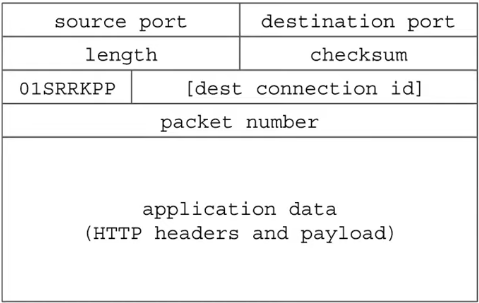
\includegraphics[width=0.45\textwidth]{fig/QUIC/quic_header.png}
    \hfill
    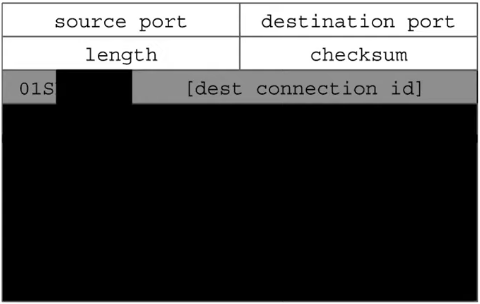
\includegraphics[width=0.45\textwidth]{fig/QUIC/quic_header_enc.png}
    \caption{\textit{Header protection} do QUIC em pacotes \textit{short header}. Fonte: adaptado de \citep{marx2020quic}.}
    \label{fig:quic_short_header_protection}
\end{figure}

\subsection{Tipos de pacotes QUIC}

O QUIC define seis tipos de pacote: \texttt{Initial}, \texttt{0-RTT}, \texttt{Handshake} e \texttt{Retry}, com \textit{long header}; \texttt{1-RTT}, com \textit{short header}; e \textit{Version Negotiation}, descrito na Seção~\ref{sec:version_negotiation_packet}. Os pacotes \texttt{Initial}, \texttt{0-RTT}, \texttt{Handshake} e \texttt{1-RTT} estão associados a um nível de criptografia, discutido na Seção~\ref{sec:quic_packet_protection}, e a um dos três espaços de números de pacote (\textit{packet number spaces}): \textit{Initial}, \textit{Handshake} e \textit{Application Data}, este último compartilhado pelos pacotes \texttt{0-RTT} e \texttt{1-RTT}. Cada espaço mantém sua própria numeração, independente dos demais, conforme discutido na Seção~\ref{sec:quic_acknowledgement}. Os pacotes \texttt{Retry} e \textit{Version Negotiation} não possuem número de pacote; o \texttt{Retry} possui apenas uma etiqueta de integridade, e o \textit{Version Negotiation} não possui proteção criptográfica.

\subsubsection{Pacotes com \textit{long header}}
\label{sec:quic_long_header_packets}

Os pacotes com \textit{long header} são utilizados durante o estabelecimento da conexão, até que os \textit{endpoints} passem a utilizar as chaves 1-RTT. Esses pacotes utilizam o cabeçalho descrito na Seção~\ref{sec:quic_long_header}, e seus tipos estão listados na Tabela~\ref{tab:quic_long_header_packets}.


\paragraph{Pacote Initial}

O pacote \texttt{Initial} transporta as primeiras mensagens do \textit{handshake} TLS, o \texttt{Client Hello} e o \texttt{ServerHello}, em \textit{frames} \texttt{CRYPTO}. Suas chaves derivam do DCID escolhido pelo cliente e de um \textit{salt} fixo definido pela versão do protocolo \citep{rfc9001}; como esses valores são públicos, qualquer observador pode decifrar os pacotes \texttt{Initial}. Essa proteção, portanto, não oferece confidencialidade, mas dificulta a injeção de pacotes por atacantes fora do caminho da conexão (\textit{off-path}). O cabeçalho do pacote \texttt{Initial} inclui ainda um campo \textit{Token}, utilizado na validação de endereço, e os datagramas que transportam pacotes \texttt{Initial} do cliente devem ter ao menos 1200 bytes. A Tabela~\ref{tab:quic_frames_tab} apresenta os demais \textit{frames} permitidos nesse pacote.

\paragraph{Pacote 0-RTT}

O pacote \texttt{0-RTT} transporta dados de aplicação enviados pelo cliente na primeira transmissão de mensagens, junto ao pacote \texttt{Initial}, antes da conclusão do \textit{handshake}. Esse pacote só pode ser utilizado na retomada de uma sessão anterior: suas chaves derivam de uma PSK (\textit{Pre-Shared Key}) obtida pelo cliente na conexão anterior, por meio de um \textit{session ticket} do TLS~1.3 \citep{rfc8446}. Os dados 0-RTT são cifrados, mas não possuem sigilo futuro (\textit{forward secrecy}) e podem ser reproduzidos por um atacante (\textit{replay}), de modo que a aplicação deve restringir seu uso a operações idempotentes. A Seção~\ref{sec:0rtt_connection_recovery} descreve o uso desses pacotes na retomada de sessão.

\paragraph{Pacote Handshake}

O pacote \texttt{Handshake} transporta, em \textit{frames} \texttt{CRYPTO}, as mensagens do \textit{handshake} TLS posteriores ao \texttt{ServerHello}: \texttt{EncryptedExtensions}, \texttt{Certificate}, \texttt{CertificateVerify} e \texttt{Finished} do servidor e a mensagem \texttt{Finished} do cliente. Esses pacotes são protegidos pelas \textit{Handshake keys}, derivadas do segredo compartilhado obtido na troca de chaves (EC)DHE (\textit{(Elliptic Curve) Diffie-Hellman Ephemeral}) realizada por meio do \texttt{ClientHello} e do \texttt{ServerHello}. Diferentemente das chaves \textit{Initial}, as \textit{Handshake keys} oferecem confidencialidade, pois dependem de um segredo conhecido apenas pelos \textit{endpoints}. A Tabela~\ref{tab:quic_frames_tab} apresenta os demais \textit{frames} permitidos nesse pacote.

\paragraph{Pacote Retry}

O pacote \texttt{Retry} é enviado pelo servidor em resposta a um pacote \texttt{Initial} do cliente, com o objetivo de validar o endereço deste antes de alocar recursos para a conexão. O pacote transporta um \textit{Retry Token}, que o cliente deve repetir no campo \textit{Token} de um novo pacote \texttt{Initial}. Ao receber o \textit{token}, o servidor confirma que o cliente recebe pacotes no endereço declarado, o que dificulta ataques com endereço de origem forjado (\textit{spoofing}). A Seção~\ref{sec:quic_connection} discute a validação de endereço. O pacote \texttt{Retry} não transporta \textit{frames} nem é cifrado, mas inclui uma \textit{Retry Integrity Tag}, calculada com uma chave fixa definida pelo RFC~9001 sobre o conteúdo do pacote e o DCID original do cliente \citep{rfc9001}. Como a chave é pública, a etiqueta não oferece autenticação, mas permite descartar pacotes corrompidos pela rede e garante que apenas uma entidade que observou o pacote \texttt{Initial} original consiga gerar um \texttt{Retry} válido.

\subsubsection{Pacote de \textit{Version Negotiation}}
\label{sec:version_negotiation_packet}

O pacote de \textit{Version Negotiation} utiliza o formato de \textit{long header} e é enviado pelo servidor em resposta a um pacote do cliente cuja versão o servidor não suporta. O pacote lista as versões aceitas pelo servidor e repete os \textit{Connection IDs} do pacote recebido, com os campos de origem e destino invertidos, o que permite ao cliente verificar que a resposta corresponde ao pacote que enviou.

Como esse pacote independe de versão, seu formato é definido pelo RFC~8999 \citep{rfc8999}, que admite \textit{Connection IDs} de até 255 bytes. O limite de 20 bytes aplica-se apenas aos pacotes do QUICv1 \citep{rfc9000}: um \textit{endpoint} descarta pacotes da versão 1 com \textit{Connection IDs} maiores, mas um servidor deve ser capaz de ler identificadores mais longos de outras versões para formar corretamente o pacote de \textit{Version Negotiation}.

\begin{figure}[!ht]
        \centering
        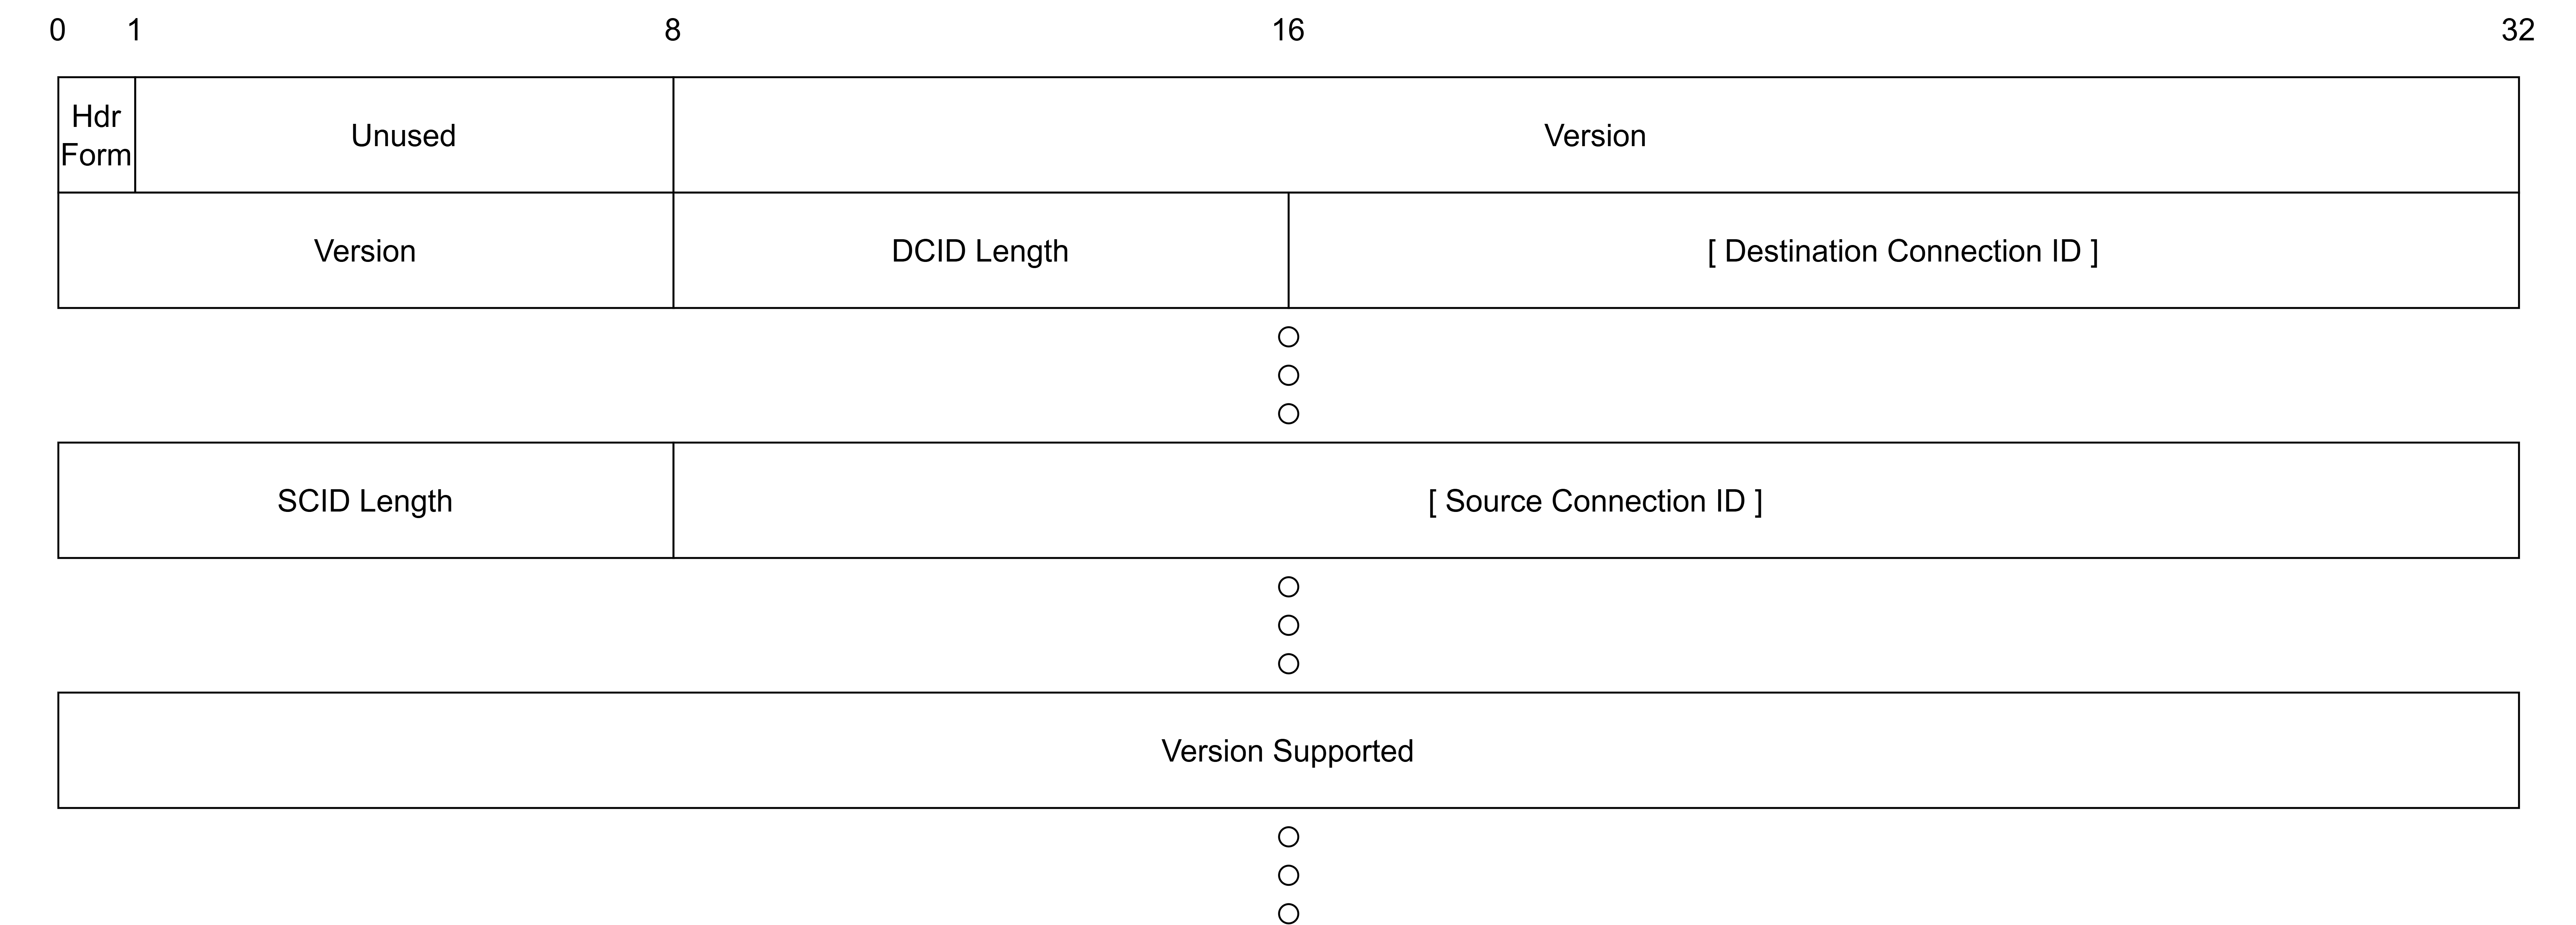
\includegraphics[width=1.0\linewidth]{fig/QUIC/quic_version_negotiation_packet.png}
        \caption{Pacote de Version Negotiation do QUIC.}
        \label{fig:quic_version_negotiation_packet}
\end{figure}

A Figura~\ref{fig:quic_version_negotiation_packet} apresenta o formato do pacote, cujos campos são descritos a seguir:

\begin{itemize}
    \item \textbf{Primeiro byte:}
    \begin{itemize}
        \item \textbf{Header Form} (1 bit): possui o valor 1, como no \textit{long header};
        \item \textbf{Unused} (7 bits): bits com valor arbitrário definido pelo servidor e ignorados pelo cliente. Quando o QUIC compartilha a porta com outros protocolos, o servidor deve atribuir o valor 1 ao bit mais significativo desse campo;
    \end{itemize}
    \item \textbf{Version} (32 bits): possui o valor \texttt{0x00000000}, reservado para identificar o pacote de \textit{Version Negotiation} e que nenhuma versão do protocolo pode utilizar;
    \item \textbf{Destination Connection ID Length} (8 bits) e \textbf{Destination Connection ID} (0 a 255 bytes): repetem o SCID do pacote recebido do cliente;
    \item \textbf{Source Connection ID Length} (8 bits) e \textbf{Source Connection ID} (0 a 255 bytes): repetem o DCID do pacote recebido do cliente;
    \item \textbf{Supported Version} (32 bits cada): lista das versões suportadas pelo servidor.
\end{itemize}

\subsubsection{Pacotes com \textit{short header}}
\label{sec:quic_short_header_packets}

Os pacotes com \textit{short header} transportam dados e informações de controle após o estabelecimento das chaves 1-RTT, conforme descrito na Seção~\ref{sec:quic_short_header}. No QUICv1, o \textit{short header} possui um único tipo de pacote, o \texttt{1-RTT}.

\paragraph{Pacote 1-RTT}

O pacote \texttt{1-RTT} pode transportar a maioria dos tipos de \textit{frame}, conforme a Tabela~\ref{tab:quic_frames_tab}, e é utilizado principalmente após a conclusão do \textit{handshake}. O servidor, entretanto, dispõe das chaves 1-RTT logo após enviar sua mensagem \texttt{Finished}, antes de receber a mensagem \texttt{Finished} do cliente, e pode enviar dados de aplicação nesse intervalo. Esses dados são denominados 0.5-RTT \citep{rfc9001}. Como o servidor ainda não verificou o \texttt{Finished} do cliente, os dados 0.5-RTT não devem depender da autenticação do cliente. Após a conclusão do \textit{handshake}, ambos os \textit{endpoints} utilizam as chaves 1-RTT.

\subsubsection{Proteção de pacotes}
\label{sec:quic_packet_protection}

Esta seção detalha a proteção aplicada aos pacotes QUIC em cada nível de criptografia, que complementa a proteção de cabeçalho descrita na Seção~\ref{sec:quic_header_protection}. Com exceção do \textit{Version Negotiation}, todos os tipos de pacote possuem algum mecanismo de proteção, descrito a seguir.

\paragraph{Initial Secrets}

Os \textit{Initial Secrets} são os segredos utilizados na proteção dos pacotes \texttt{Initial}. O QUIC calcula um segredo inicial pela função HKDF-Extract, a partir de um \textit{salt} fixo definido para a versão e do DCID escolhido pelo cliente em seu primeiro pacote \texttt{Initial} \citep{rfc9001}. Desse segredo derivam dois segredos distintos, um para cada sentido da comunicação, obtidos com os rótulos \texttt{client in} e \texttt{server in}. Se o servidor responder com um pacote \texttt{Retry}, o cliente recalcula os segredos com o novo DCID, escolhido pelo servidor no campo SCID do \texttt{Retry}.

\paragraph{0-RTT Keys}

As chaves 0-RTT derivam da PSK obtida em uma sessão anterior com o mesmo servidor e, portanto, são distintas das chaves 1-RTT, que dependem também do segredo (EC)DHE negociado na conexão atual. Como dependem apenas da PSK, as chaves 0-RTT não oferecem \textit{forward secrecy}: o comprometimento da PSK expõe os dados 0-RTT de todas as conexões que a utilizaram. Além disso, um atacante pode reenviar pacotes 0-RTT capturados (\textit{replay}), fazendo com que o servidor processe a mesma requisição mais de uma vez. Por isso, o RFC~9001 \citep{rfc9001} exige que o protocolo de aplicação defina quais operações podem ser enviadas em 0-RTT, em geral apenas as idempotentes. Os pacotes 0-RTT aceitam apenas parte dos tipos de \textit{frame}, conforme a Tabela~\ref{tab:quic_frames_tab}, e o cliente pode enviá-los até obter as chaves 1-RTT.

\paragraph{Handshake Keys}

As \textit{Handshake Keys} derivam do \textit{Handshake Secret} do TLS~1.3, obtido a partir do segredo compartilhado da troca de chaves (EC)DHE \citep{rfc8446}. Desse segredo, o TLS deriva um segredo de tráfego para cada sentido, com os rótulos \texttt{c hs traffic} e \texttt{s hs traffic}, que incorporam o \textit{hash} das mensagens \texttt{ClientHello} e \texttt{ServerHello}. A esses segredos, o QUIC aplica os rótulos \texttt{quic key}, \texttt{quic iv} e \texttt{quic hp} para obter as chaves de proteção do pacote, o IV e a chave de proteção do cabeçalho \citep{rfc9001}. Essas chaves protegem apenas os pacotes \texttt{Handshake}.

\paragraph{Retry Integrity Tag}
\label{sec:quic_retry_integrity_tag}

A \textit{Retry Integrity Tag} é um campo de 128 bits que encerra o pacote \texttt{Retry}. O servidor a calcula com o algoritmo AEAD\_AES\_128\_GCM, que utiliza uma chave e um \textit{nonce} fixos definidos pelo RFC~9001 \citep{rfc9001}, um texto claro vazio e, como dados associados, um pseudopacote formado pelo DCID original do cliente e pelo conteúdo do \texttt{Retry}. Como a chave é pública, a etiqueta não envolve derivação de chaves nem oferece confidencialidade ou autenticação, mas protege o pacote contra corrupção acidental e contra atacantes que não observaram o pacote \texttt{Initial} original.

\paragraph{1-RTT Keys}

As \textit{1-RTT Keys} derivam do \textit{Master Secret} do TLS~1.3, que, por sua vez, deriva do \textit{Handshake Secret} \citep{rfc8446}. Do \textit{Master Secret}, o TLS obtém um segredo de tráfego de aplicação para cada sentido, com os rótulos \texttt{c ap traffic} e \texttt{s ap traffic}, que incorporam o \textit{hash} das mensagens do \textit{handshake} até o \texttt{Finished} do servidor. Assim como nas \textit{Handshake Keys}, o QUIC aplica a esses segredos os rótulos \texttt{quic key}, \texttt{quic iv} e \texttt{quic hp} \citep{rfc9001}. Na atualização de chaves sinalizada pelo bit \textit{Key Phase}, o QUIC deriva um novo segredo com o rótulo \texttt{quic ku}, sem alterar a chave de proteção do cabeçalho. As \textit{1-RTT Keys} protegem exclusivamente os pacotes \texttt{1-RTT}.

\subsubsection{\textit{Frames} do QUIC}

Com exceção dos pacotes \texttt{Retry} e \textit{Version Negotiation}, o \textit{payload} de um pacote QUIC é composto por uma sequência de \textit{frames}. Cada tipo de pacote admite apenas determinados tipos de \textit{frame}, conforme a Tabela~\ref{tab:quic_frames_tab}. A função de cada tipo de \textit{frame} é definida no RFC~9000 \citep{rfc9000} e não é detalhada neste trabalho.


\begin{table}[!ht]
\centering
\begin{tabular}{|c|l|l|}
\hline
\textbf{Valor} & \textbf{Tipo de \textit{frame}} & \textbf{Pacotes} \\ \hline
0x00       & PADDING                 & Initial, 0-RTT, Handshake, 1-RTT \\ \hline
0x01       & PING                    & Initial, 0-RTT, Handshake, 1-RTT \\ \hline
0x02--0x03 & ACK                     & Initial, Handshake, 1-RTT \\ \hline
0x04       & RESET\_STREAM            & 0-RTT, 1-RTT \\ \hline
0x05       & STOP\_SENDING            & 0-RTT, 1-RTT \\ \hline
0x06       & CRYPTO                  & Initial, Handshake, 1-RTT \\ \hline
0x07       & NEW\_TOKEN               & 1-RTT \\ \hline
0x08--0x0f & STREAM                  & 0-RTT, 1-RTT \\ \hline
0x10       & MAX\_DATA                & 0-RTT, 1-RTT \\ \hline
0x11       & MAX\_STREAM\_DATA        & 0-RTT, 1-RTT \\ \hline
0x12--0x13 & MAX\_STREAMS             & 0-RTT, 1-RTT \\ \hline
0x14       & DATA\_BLOCKED            & 0-RTT, 1-RTT \\ \hline
0x15       & STREAM\_DATA\_BLOCKED    & 0-RTT, 1-RTT \\ \hline
0x16--0x17 & STREAMS\_BLOCKED         & 0-RTT, 1-RTT \\ \hline
0x18       & NEW\_CONNECTION\_ID      & 0-RTT, 1-RTT \\ \hline
0x19       & RETIRE\_CONNECTION\_ID   & 1-RTT \\ \hline
0x1a       & PATH\_CHALLENGE          & 0-RTT, 1-RTT \\ \hline
0x1b       & PATH\_RESPONSE           & 1-RTT \\ \hline
0x1c       & CONNECTION\_CLOSE        & Initial, 0-RTT, Handshake, 1-RTT \\ \hline
0x1d       & CONNECTION\_CLOSE        & 0-RTT, 1-RTT \\ \hline
0x1e       & HANDSHAKE\_DONE          & 1-RTT \\ \hline
\end{tabular}
\caption{Tipos de \textit{frame} do QUIC e pacotes que podem transportá-los. Fonte: adaptado de \citep{rfc9000}.}
\label{tab:quic_frames_tab}
\end{table}


\section{Conexão do QUIC}
\label{sec:quic_connection}

O estabelecimento de conexão do QUIC segue diferentes fluxos, conforme o estado prévio dos \textit{endpoints} e os pacotes recebidos. Esta seção descreve o \textit{handshake} 1-RTT, utilizado como caso base, e suas variações:

\begin{itemize}
    \item A Seção~\ref{sec:quic_connection_steps} detalha as etapas do \textit{handshake} 1-RTT do QUICv1;
    \item A Seção~\ref{sec:0rtt_connection_recovery} descreve a retomada de sessão com dados 0-RTT;
    \item A Seção~\ref{sec:quic_version_negotiation} descreve a negociação da versão do protocolo entre os \textit{endpoints};
    \item A Seção~\ref{sec:quic_address_validation} descreve a validação de endereço, que mitiga ataques de \textit{spoofing} e de amplificação;
    \item A Seção~\ref{sec:connection_ids_operation} descreve o funcionamento dos \textit{Connection IDs}.
\end{itemize}

A Seção~\ref{sec:quic_connection_steps} descreve o \textit{handshake} TLS apenas no nível necessário à compreensão do QUIC; o funcionamento detalhado do TLS~1.3 é definido no RFC~8446 \citep{rfc8446}.

\subsection{Etapas de conexão do QUIC}
\label{sec:quic_connection_steps}

No fluxo padrão, denominado \textit{handshake} 1-RTT, o QUIC combina o estabelecimento da conexão de transporte com o \textit{handshake} TLS~1.3: os parâmetros de transporte de cada \textit{endpoint} são trocados em uma extensão do próprio TLS \citep{rfc9001}. Assim, o cliente pode enviar dados de aplicação após um único RTT, enquanto a combinação de TCP e TLS~1.3 exige dois RTTs: um para o \textit{3-way handshake} do TCP e outro para o \textit{handshake} TLS. A Figura~\ref{fig:quic_vs_tcptls} compara os dois fluxos.

\begin{figure}[!ht]
        \centering
        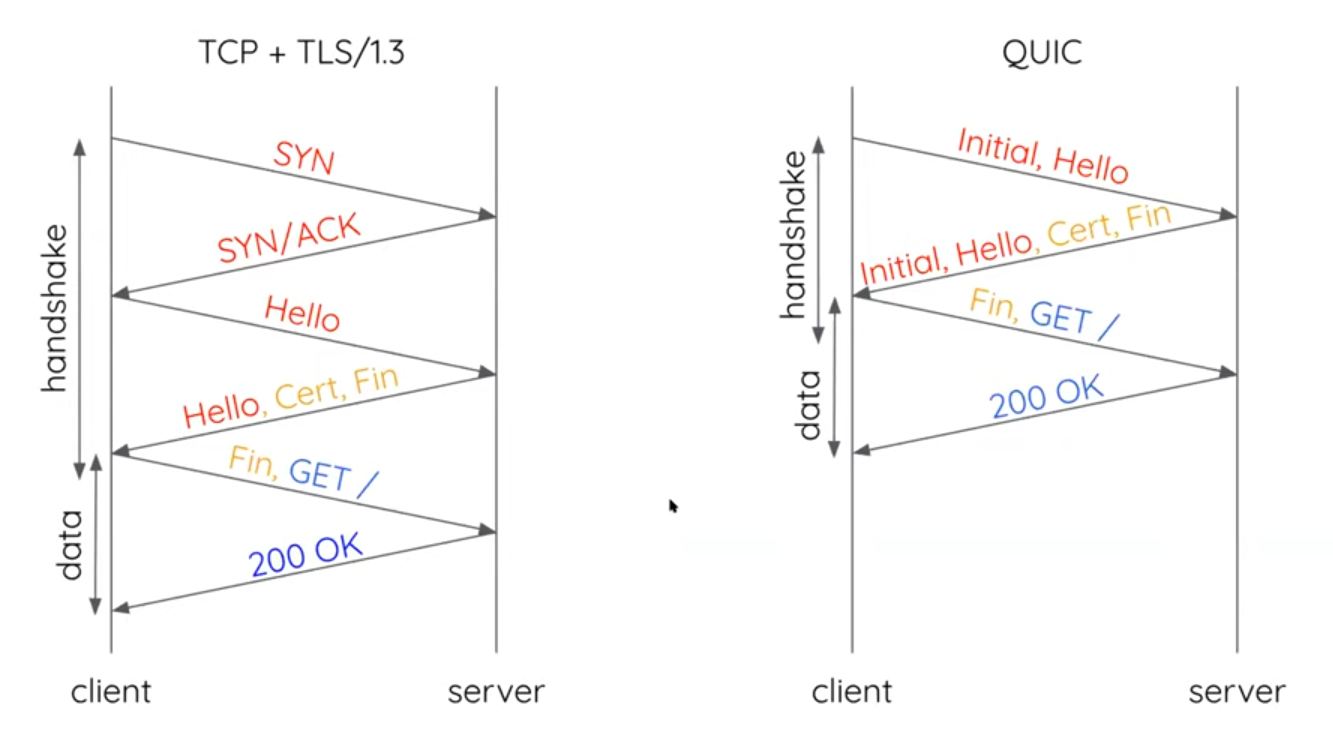
\includegraphics[width=0.85\linewidth]{fig/QUIC/quic_vs_tcptls_cmp.png}
        \caption{Comparação entre conexões do TCP/TLS e QUIC. Fonte: adaptado de \citep{marx2020quic}.}
        \label{fig:quic_vs_tcptls}
\end{figure}

O \textit{handshake} 1-RTT ocorre da seguinte forma. O cliente envia um pacote \texttt{Initial} com a mensagem \texttt{ClientHello}, que contém sua parcela da troca de chaves (EC)DHE e seus parâmetros de transporte.

O servidor responde com um pacote \texttt{Initial}, que contém a confirmação de recebimento (\textit{frame} \texttt{ACK}) do pacote do cliente e a mensagem \texttt{ServerHello}, e com um pacote \texttt{Handshake}, que contém as mensagens \texttt{EncryptedExtensions}, \texttt{Certificate}, \texttt{CertificateVerify} e \texttt{Finished}. Opcionalmente, o servidor envia também um pacote \texttt{1-RTT} com dados 0.5-RTT, discutidos na Seção~\ref{sec:quic_short_header_packets}. Esses pacotes podem ser agrupados em um mesmo datagrama UDP (\textit{coalescing}).

O cliente confirma o recebimento dos pacotes \texttt{Initial} e \texttt{Handshake} do servidor e conclui sua parte do \textit{handshake} TLS ao enviar a mensagem \texttt{Finished} em um pacote \texttt{Handshake}. A partir desse momento, o cliente pode enviar dados de aplicação em pacotes \texttt{1-RTT}.

Ao receber o \texttt{Finished} do cliente, o servidor considera o \textit{handshake} concluído e confirmado e envia ao cliente um \textit{frame} \texttt{HANDSHAKE\_\allowbreak{}DONE}. O cliente, por sua vez, considera o \textit{handshake} confirmado ao receber esse \textit{frame}. A confirmação permite que os \textit{endpoints} descartem as chaves de \textit{Handshake} e é pré-requisito para operações como a migração de conexão, discutida na Seção~\ref{sec:quic_connection_migration}. A Figura~\ref{fig:quic_connection_steps_time_diagram} ilustra esse fluxo.

\begin{figure}[!ht]
        \centering
        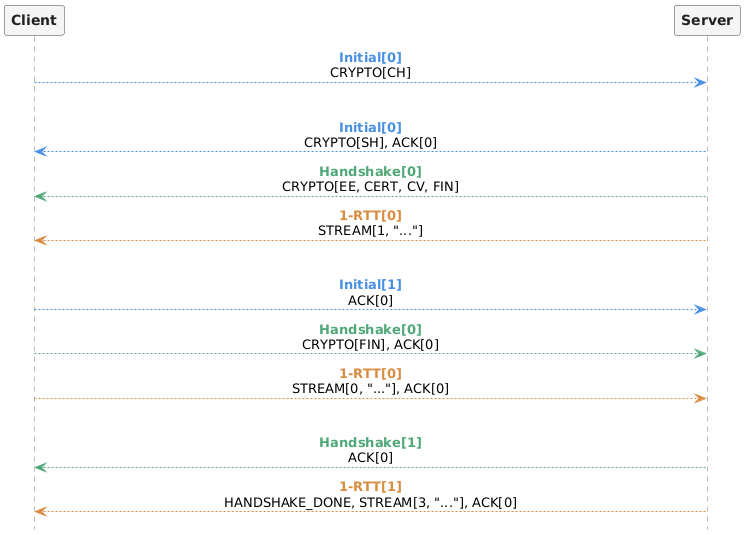
\includegraphics[width=0.9\linewidth]{fig/QUIC/quic_connection_steps.png}
        \caption{Diagrama de tempo do \textit{handshake} 1-RTT do QUIC. Fonte: elaborado com base em \citep{rfc9000}.}
        \label{fig:quic_connection_steps_time_diagram}
\end{figure}

\subsection{Retomada de sessão (0-RTT)}
\label{sec:0rtt_connection_recovery}


A retomada de sessão permite que o cliente reaproveite o estado criptográfico de uma conexão anterior com o mesmo servidor. Nessa conexão anterior, o servidor envia ao cliente um \textit{session ticket} do TLS~1.3, a partir do qual o cliente obtém uma PSK. Em uma nova conexão, o cliente deriva dessa PSK as chaves 0-RTT e envia dados de aplicação, em \textit{frames} \texttt{STREAM}, no primeiro voo de mensagens, junto ao pacote \texttt{Initial}, sem aguardar nenhum RTT. O restante do \textit{handshake} segue o fluxo 1-RTT. A Figura~\ref{fig:quic0rtt_vs_tcptls} compara a retomada de sessão no QUIC e no TCP com TLS, e a Figura~\ref{fig:quic_connection_resumption_time_diagram} ilustra o fluxo de pacotes.

\begin{figure}[!ht]
        \centering
        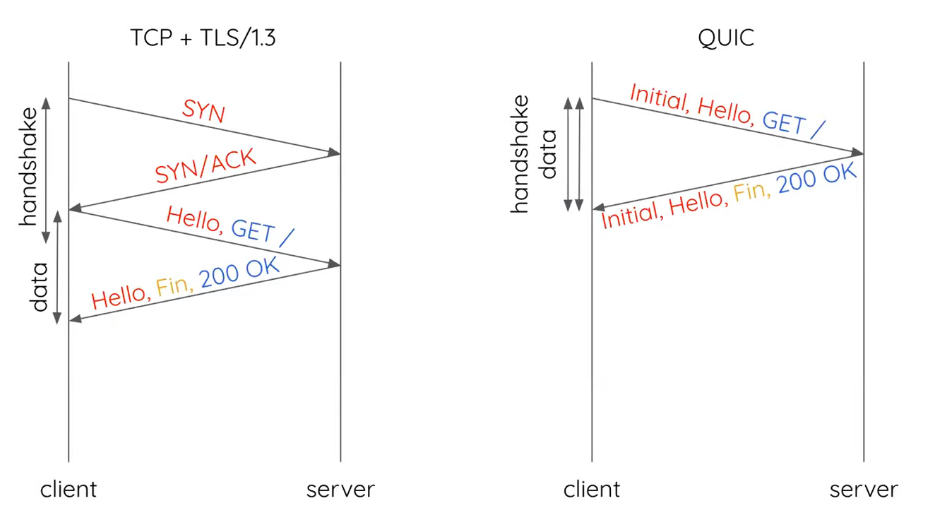
\includegraphics[width=0.8\linewidth]{fig/QUIC/quic0rtt_vs_tcptls_cmp.png}
        \caption{Comparação da retomada de sessão no QUIC (0-RTT) e no TCP com TLS. Fonte: adaptado de \citep{marx2020quic}.}
        \label{fig:quic0rtt_vs_tcptls}
\end{figure}

\begin{figure}[!ht]
        \centering
        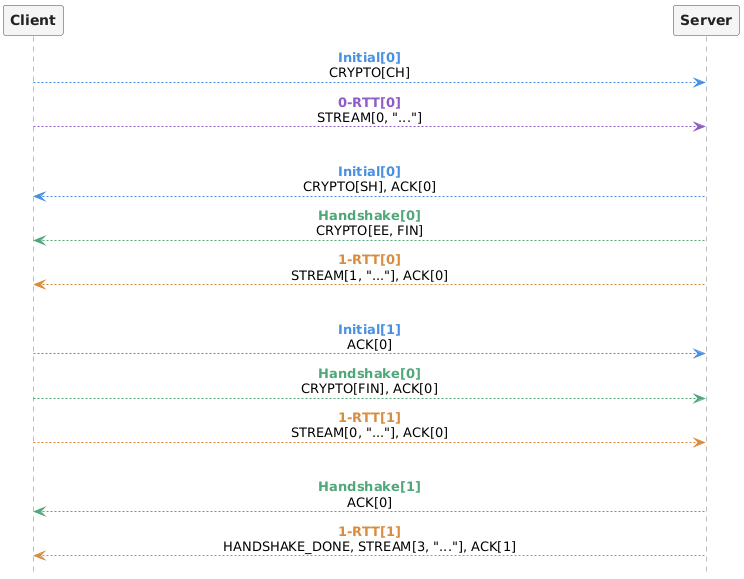
\includegraphics[width=0.7\linewidth]{fig/QUIC/quic_connection_resumption.png}
        \caption{Diagrama de tempo da retomada de sessão do QUIC. Fonte: elaborado com base em \citep{rfc9000}.}
        \label{fig:quic_connection_resumption_time_diagram}
\end{figure}


Os dados 0-RTT, entretanto, estão sujeitos a ataques de \textit{replay}, mencionados na Seção~\ref{sec:quic_packet_protection}: um atacante pode capturar um pacote 0-RTT e reenviá-lo ao servidor, que não consegue distinguir a repetição de uma nova requisição, pois o pacote permanece criptograficamente válido. O critério para decidir o que pode ser enviado em 0-RTT é a idempotência. Operações cuja repetição produz o mesmo efeito de uma única execução, como a leitura de dados, podem ser processadas mais de uma vez sem prejuízo, enquanto operações não idempotentes, como uma compra ou uma transferência financeira, podem ter seus efeitos duplicados. Por isso, protocolos de aplicação como o HTTP/3 definem mecanismos próprios de proteção: o servidor pode responder a uma requisição recebida em 0-RTT com o código de status \texttt{425 Too Early} \citep{rfc8470}, o que leva o cliente a repeti-la após a conclusão do \textit{handshake}.

\subsection{Negociação de versão}
\label{sec:quic_version_negotiation}

A negociação de versão permite que cliente e servidor estabeleçam uma versão comum do QUIC. Ao receber do cliente um pacote com uma versão que não suporta, o servidor responde com um pacote de \textit{Version Negotiation}, que lista as versões aceitas. O cliente então seleciona uma dessas versões e inicia uma nova tentativa de conexão com um novo pacote \texttt{Initial}, o que acrescenta um RTT ao estabelecimento da conexão, conforme a Figura~\ref{fig:quic_version_negotiation_time_diagram}. O servidor não mantém estado durante esse processo e pode limitar o número de pacotes de \textit{Version Negotiation} que envia \citep{rfc9000}. Como esse pacote não é autenticado, o QUICv1 não protege a escolha de versão contra ataques de \textit{downgrade}; o RFC~9368 \citep{rfc9368} define um mecanismo complementar para essa proteção.

\begin{figure}[!ht]
        \centering
        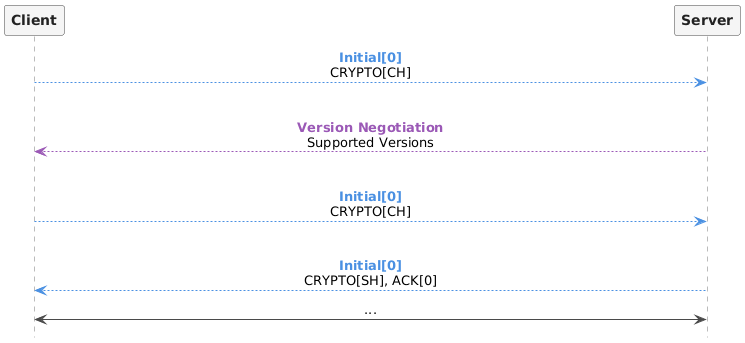
\includegraphics[width=0.7\linewidth]{fig/QUIC/quic_version_negotiation.png}
        \caption{Diagrama de tempo da negociação de versão do QUICv1. Fonte: elaborado com base em \citep{rfc9000}.}
        \label{fig:quic_version_negotiation_time_diagram}
\end{figure}

\subsection{Validação de endereço}
\label{sec:quic_address_validation}

A validação de endereço permite ao servidor confirmar que o cliente recebe pacotes no endereço de origem declarado \citep{rfc9000}. O mecanismo impede que o servidor seja utilizado em ataques de amplificação, nos quais o atacante forja o endereço de origem dos pacotes com o endereço da vítima (\textit{spoofing}), de modo que o servidor envie à vítima um volume de tráfego superior ao gerado pelo atacante. Para isso, o servidor limita os dados enviados a endereços ainda não validados ou valida o endereço antes de prosseguir com o \textit{handshake}. A validação não oferece garantias sobre o conteúdo transmitido; ela apenas confirma que o cliente recebe as respostas no endereço declarado.

Antes da validação, o servidor não pode enviar a um endereço mais do que o triplo dos bytes recebidos desse endereço \citep{rfc9000}. Esse limite de amplificação restringe o tráfego que um atacante consegue direcionar a uma vítima por meio do servidor.

Esse limite pode causar um impasse (\textit{deadlock}): se o servidor o atingir antes de concluir o envio de suas mensagens de \textit{handshake} e as confirmações do cliente se perderem, nenhum dos \textit{endpoints} envia novos pacotes. Para evitar essa situação, o cliente envia pacotes de sondagem (\textit{probe packets}) sempre que seu temporizador de PTO (\textit{Probe Timeout}) expira, mesmo sem dados a transmitir, até ter a garantia de que o servidor validou seu endereço \citep{rfc9002}. Cada pacote recebido amplia a margem de envio do servidor.

Para que o servidor disponha de margem suficiente desde a primeira troca, os datagramas UDP que transportam pacotes \texttt{Initial} do cliente devem ter ao menos 1200 bytes, completados com \textit{frames} \texttt{PADDING} quando necessário. Assim, o servidor pode responder com até 3600 bytes antes de validar o endereço do cliente.

Algumas formas de validação decorrem do próprio \textit{handshake}. O servidor considera validado o endereço do cliente ao receber dele um pacote \texttt{Handshake}, pois o cliente só consegue gerar esse pacote após processar o pacote \texttt{Initial} do servidor. O servidor também pode considerar o endereço validado quando o cliente utiliza um \textit{Connection ID} escolhido pelo servidor com ao menos 64 bits de entropia, já que o cliente só conhece esse identificador se recebeu os pacotes do servidor.

Quando o servidor deseja validar o endereço do cliente antes de prosseguir com o \textit{handshake}, ele responde ao primeiro pacote \texttt{Initial} com um pacote \texttt{Retry} que contém um \textit{token} \citep{rfc9000}. O cliente deve repetir esse \textit{token} no campo \textit{Token} de seu novo pacote \texttt{Initial}, o que comprova o recebimento do \texttt{Retry} no endereço declarado. Como apenas o servidor que emitiu o \textit{token} o valida, seu formato não é padronizado; o servidor deve apenas impedir que outra entidade o forje, em geral por meio de autenticação criptográfica que vincula o \textit{token} ao endereço do cliente. Esse mecanismo acrescenta um RTT ao estabelecimento da conexão, conforme a Figura~\ref{fig:quic_retry_with_token}.

\begin{figure}[!ht]
        \centering
        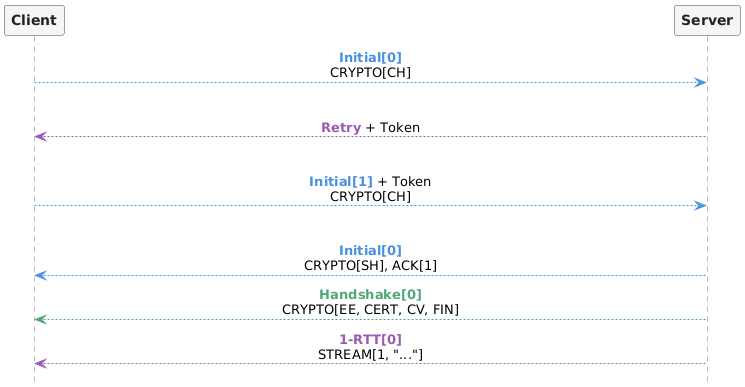
\includegraphics[width=0.7\linewidth]{fig/QUIC/quic_retry_with_token.png}
        \caption{Diagrama de tempo da validação de endereço com pacote \texttt{Retry}. Fonte: elaborado com base em \citep{rfc9000}.}
        \label{fig:quic_retry_with_token}
\end{figure}
 
O servidor também pode fornecer ao cliente, durante uma conexão estabelecida, um \textit{token} por meio do \textit{frame} \texttt{NEW\_\allowbreak{}TOKEN} \citep{rfc9000}. O cliente inclui esse \textit{token} no pacote \texttt{Initial} de uma conexão futura, o que permite ao servidor validar o endereço sem o RTT adicional do \texttt{Retry} e, assim, enviar respostas maiores, como as respostas a requisições 0-RTT, sem as restrições do limite de amplificação.

\subsection{Funcionamento dos \textit{Connection IDs}}
\label{sec:connection_ids_operation}

Os \textit{Connection IDs} permitem que o \textit{endpoint} receptor associe cada pacote à conexão correta independentemente dos endereços e das portas das camadas inferiores, que podem mudar ao longo da conexão. Cada \textit{endpoint} escolhe os identificadores pelos quais deseja ser endereçado: o DCID de um pacote corresponde ao identificador escolhido pelo receptor, e o SCID, ao identificador escolhido pelo emissor (Seção~\ref{sec:quic_headers}).

Ao longo da conexão, cada \textit{endpoint} fornece ao outro novos \textit{Connection IDs} por meio de \textit{frames} \texttt{NEW\_\allowbreak{}CONNECTION\_\allowbreak{}ID} e solicita o descarte dos antigos com \textit{frames} \texttt{RETIRE\_\allowbreak{}CONNECTION\_\allowbreak{}ID} \citep{rfc9000}. A troca de identificadores, em especial após uma migração de conexão, impede que um observador externo associe à mesma conexão pacotes enviados por caminhos diferentes. Para isso, um identificador não deve permitir sua correlação com os demais identificadores da mesma conexão, o que leva as implementações a gerá-los com um gerador de números pseudoaleatórios criptograficamente seguro (CSPRNG, \textit{Cryptographically Secure Pseudorandom Number Generator}).

Um \textit{endpoint} pode utilizar \textit{Connection IDs} de tamanho zero quando o endereço e a porta bastam para identificar a conexão. Nesse caso, porém, o \textit{endpoint} depende desses valores para associar os pacotes e perde o suporte a recursos como a migração de conexão e a tolerância a \textit{NAT rebinding}, relevantes para as técnicas de \textit{hole punching} discutidas na Seção~\ref{sec:quic_hole_punching}.

\cgk{Confirmar quando escrever sobre QUIC holepunching se isso realmente se aplica}

O ciclo de vida dos \textit{Connection IDs}, incluindo a emissão de novos identificadores e o momento de seu descarte, é definido no RFC~9000 \citep{rfc9000} e não é detalhado neste trabalho.

\section{Comunicação do QUIC}

Esta seção apresenta os mecanismos de comunicação entre os \textit{endpoints} de uma conexão QUIC. O protocolo multiplexa, em uma mesma conexão, \textit{streams} independentes entre si, e oferece entrega confiável e controle de fluxo. Esses mecanismos são descritos nas seguintes seções:

\begin{itemize}
    \item A Seção~\ref{sec:quic_streams} descreve a criação e o gerenciamento de \textit{streams};
    \item A Seção~\ref{sec:quic_acknowledgement} descreve os espaços de números de pacote e os mecanismos de confirmação de recebimento e de retransmissão;
    \item A Seção~\ref{sec:quic_flow_control} descreve o controle de fluxo;
    \item A Seção~\ref{sec:quic_connection_migration} descreve a migração de conexão após a mudança de endereço IP ou de porta de um dos \textit{endpoints}.
\end{itemize}

\subsection{\textit{Streams} do QUIC}
\label{sec:quic_streams}

Uma \textit{stream} é um canal ordenado de bytes dentro de uma conexão QUIC e pode ser unidirecional ou bidirecional \citep{rfc9000}. Cada \textit{stream} é identificada por um \textit{Stream ID}, um inteiro de 62 bits cujos dois bits menos significativos codificam o tipo da \textit{stream}: o bit menos significativo indica qual \textit{endpoint} a iniciou, e o segundo indica se ela é bidirecional ou unidirecional, conforme a Tabela~\ref{tab:quic_stream_types}. Assim, cada tipo dispõe de $2^{60}$ identificadores, atribuídos em incrementos de 4; as \textit{streams} bidirecionais iniciadas pelo cliente, por exemplo, recebem os identificadores 0, 4, 8 e assim por diante.

\begin{table}[ht]
    \centering
    \begin{tabular}{|c|l|}
        \hline
        \textbf{Bits} & \textbf{Tipo de \textit{stream}} \\
        \hline
        0x00 & Iniciada pelo cliente, bidirecional \\
        0x01 & Iniciada pelo servidor, bidirecional \\
        0x02 & Iniciada pelo cliente, unidirecional \\
        0x03 & Iniciada pelo servidor, unidirecional \\
        \hline
    \end{tabular}
    \caption{Tipos de \textit{stream} codificados nos dois bits menos significativos do \textit{Stream ID}. Fonte: \citep{rfc9000}.}
    \label{tab:quic_stream_types}
\end{table}

As \textit{streams} transportam dados de aplicação e podem ser encerradas normalmente pelo emissor, por meio do bit FIN do \textit{frame} \texttt{STREAM}, interrompidas pelo emissor, com o \textit{frame} \texttt{RESET\_\allowbreak{}STREAM}, ou ter sua recepção cancelada pelo receptor, com o \textit{frame} \texttt{STOP\_\allowbreak{}SENDING}. O QUIC garante a entrega confiável e ordenada dos bytes dentro de cada \textit{stream}, mas não impõe ordem entre \textit{streams} distintas. Assim, a perda de um pacote atrasa apenas as \textit{streams} cujos dados ele transportava, enquanto as demais continuam a entregar dados à aplicação, como ilustra a Figura~\ref{fig:quic_no_holb}. Esse mecanismo elimina o \textit{Head-of-Line Blocking} entre fluxos presente no HTTP/2 sobre TCP. O QUICv1 não define um esquema de priorização de \textit{streams}, mas recomenda que as implementações permitam à aplicação indicar a prioridade relativa de cada uma \citep{rfc9000}.

\begin{figure}[!ht]
        \centering
        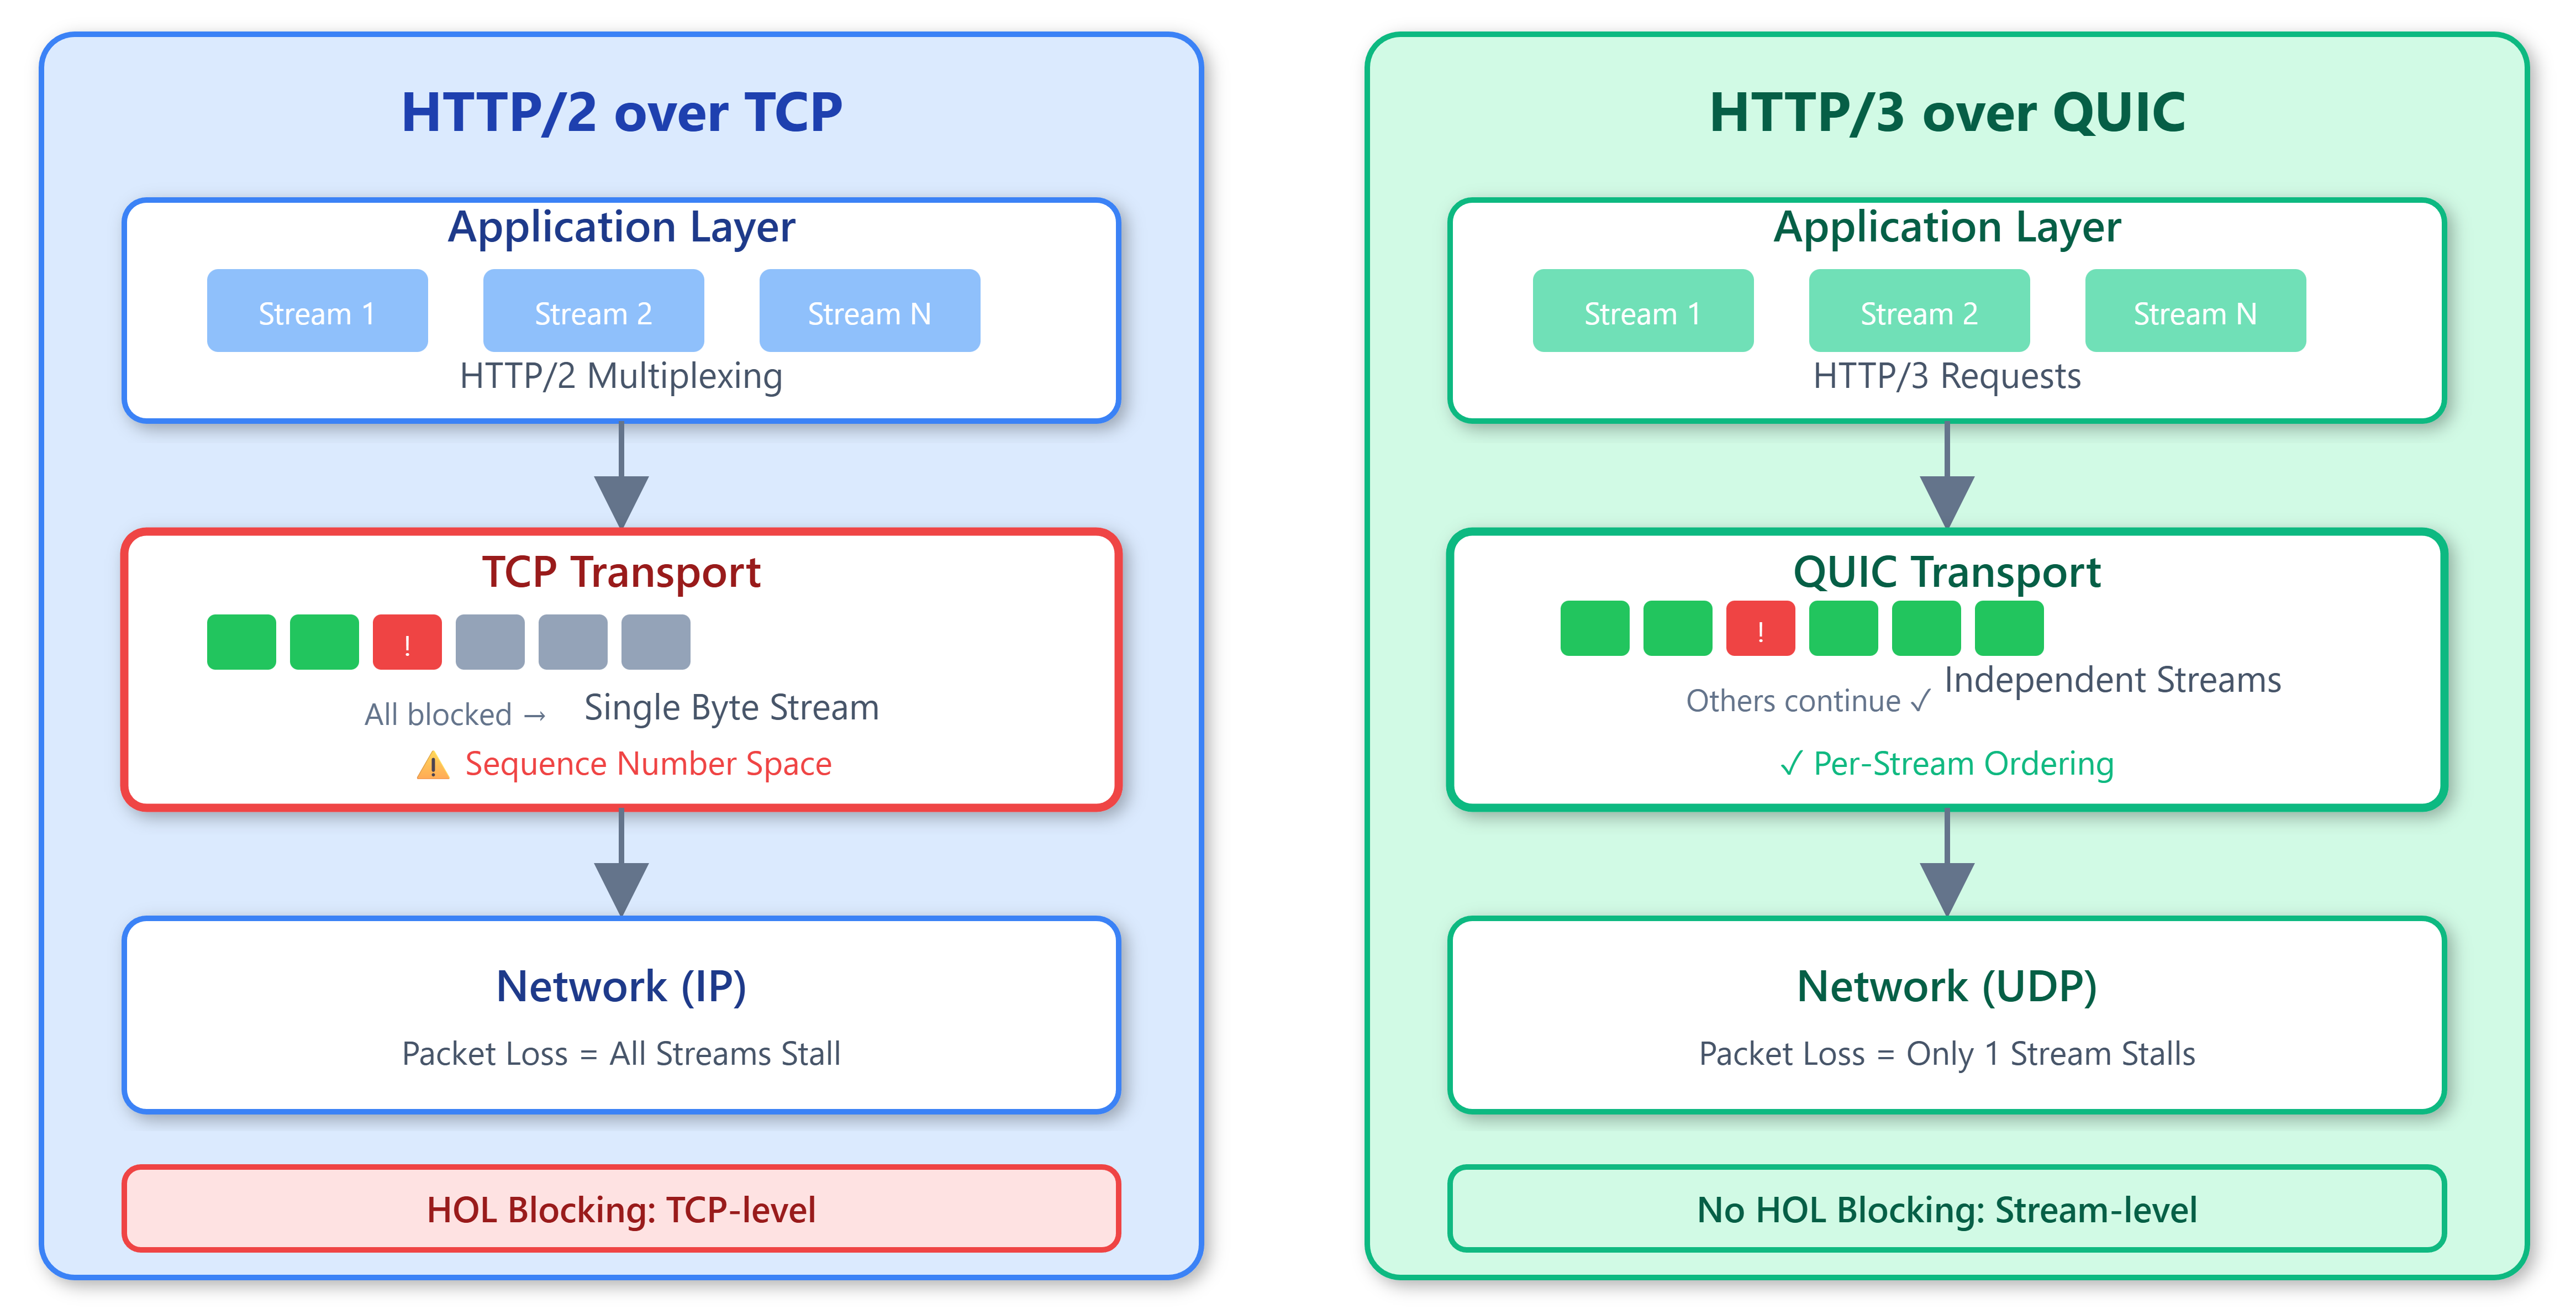
\includegraphics[width=0.9\linewidth]{fig/QUIC/quic_no_holb.png}
        \caption{Ausência de \textit{Head-of-Line Blocking} entre \textit{streams} no QUIC.}
        \label{fig:quic_no_holb}
\end{figure}

O RFC~9000 \citep{rfc9000} descreve o ciclo de vida de uma \textit{stream} por meio de duas máquinas de estados: uma para a parte de envio e outra para a parte de recepção. Em cada \textit{endpoint}, uma \textit{stream} unidirecional utiliza apenas uma dessas máquinas, enquanto uma \textit{stream} bidirecional utiliza ambas. Essas máquinas de estados servem apenas como referência: as implementações podem modelar seus estados internos de outra forma, desde que o comportamento observável seja consistente com a especificação. O detalhamento desses estados está fora do escopo deste trabalho.

\subsection{Confirmação de recebimento}
\label{sec:quic_acknowledgement}

Como descrito na Seção~\ref{sec:quic_packets}, um pacote QUIC pode conter vários \textit{frames}. Para fins de confirmação de recebimento, o pacote herda propriedades dos \textit{frames} que contém \citep{rfc9002}:

\begin{itemize}
    \item \textbf{Ack-eliciting:} pacote que contém ao menos um \textit{frame} diferente de \texttt{ACK}, \texttt{PADDING} e \texttt{CONNECTION\_\allowbreak{}CLOSE}. O receptor deve confirmar esse pacote imediatamente nos espaços \textit{Initial} e \textit{Handshake} e, no espaço \textit{Application Data}, em até \textit{max\_\allowbreak{}ack\_\allowbreak{}delay}, valor anunciado nos parâmetros de transporte;
    \item \textbf{Non-ack-eliciting:} pacote que contém apenas \textit{frames} \texttt{ACK}, \texttt{PADDING} ou \texttt{CONNECTION\_\allowbreak{}CLOSE}. O receptor não envia uma confirmação motivada apenas por esse pacote, mas o inclui nos intervalos do próximo \textit{frame} \texttt{ACK} que enviar por outro motivo.
\end{itemize}

Dessa forma, um pacote \textit{non-ack-eliciting} pode nunca ser confirmado, caso o receptor não tenha outro motivo para enviar um \textit{frame} \texttt{ACK}. A Tabela~\ref{tab:quic_ack_rules} resume as regras de envio de confirmações.

\begin{table}[ht]
    \centering
    \begin{tabular}{|p{0.72\textwidth}|c|}
        \hline
        \textbf{Situação} & \textbf{Permitido} \\
        \hline
        Responder a um pacote \textit{non-ack-eliciting} com um pacote \textit{non-ack-eliciting} enviado apenas para confirmá-lo & Não \\
        \hline
        Incluir um \textit{frame} \texttt{ACK} em um pacote que já seria enviado por outro motivo & Sim \\
        \hline
        Adiar a confirmação de um pacote \textit{non-ack-eliciting} até o recebimento de um pacote \textit{ack-eliciting} & Sim \\
        \hline
        Confirmar um pacote \textit{ack-eliciting} do espaço \textit{Application Data} em até \textit{max\_\allowbreak{}ack\_\allowbreak{}delay} & Sim \\
        \hline
    \end{tabular}
    \caption{Regras para o envio de confirmações no QUIC. Fonte: elaborado com base em \citep{rfc9000}.}
    \label{tab:quic_ack_rules}
\end{table}

Esse atraso permite ao receptor confirmar vários pacotes com um único \textit{frame} \texttt{ACK}, o que reduz a sobrecarga de confirmações.

No QUIC, a retransmissão não reenvia pacotes, mas as informações neles contidas, em novos pacotes com novos números \citep{rfc9002}. Cada tipo de \textit{frame} segue uma regra própria: os dados de \textit{streams} são reenviados em novos \textit{frames} \texttt{STREAM}, enquanto informações obsoletas, como \textit{frames} \texttt{ACK} antigos, não são retransmitidas. Como os números de pacote nunca se repetem em um mesmo espaço de numeração, o emissor distingue a confirmação de uma transmissão original da confirmação de uma retransmissão, ambiguidade presente no TCP. Essa regra também evita a reutilização de \textit{nonces} na proteção de pacotes (Seção~\ref{sec:quic_packet_protection}). A Seção~\ref{sec:quic_packet_numbers} discute os espaços de números de pacote; os algoritmos de detecção de perda e de retransmissão, definidos no RFC~9002 \citep{rfc9002}, estão fora do escopo deste trabalho.

Os \textit{frames} \texttt{ACK} descrevem intervalos de números de pacote recebidos (\textit{ACK Ranges}), e cada novo \textit{frame} \texttt{ACK} repete os intervalos já informados enquanto o receptor não souber que o emissor os recebeu, ou seja, até que o pacote que transportava esse \textit{frame} \texttt{ACK} seja confirmado \citep{rfc9000}. Assim, a perda de um pacote com um \textit{frame} \texttt{ACK} não exige retransmissão, pois o \textit{frame} \texttt{ACK} seguinte contém as mesmas informações. Como esses intervalos poderiam crescer indefinidamente, o receptor pode deixar de informar intervalos antigos para limitar o tamanho do \textit{frame}, ao custo de possíveis retransmissões desnecessárias pelo emissor.

\subsubsection{Números de pacote do QUIC}
\label{sec:quic_packet_numbers}

Os números de pacote variam de 0 a $2^{62}-1$, mas o cabeçalho transporta apenas seus bits menos significativos, em um campo de 1 a 4 bytes \citep{rfc9000}. O emissor escolhe o tamanho desse campo de modo a cobrir o dobro do intervalo entre o número do pacote atual e o maior número confirmado pelo receptor, e o receptor reconstrói o número completo a partir do maior número já recebido. Os números de pacote são organizados em três espaços:

\begin{itemize}
    \item \textbf{Initial:} pacotes \texttt{Initial};
    \item \textbf{Handshake:} pacotes \texttt{Handshake};
    \item \textbf{Application Data:} pacotes \texttt{0-RTT} e \texttt{1-RTT}.
\end{itemize}

Cada espaço possui numeração própria e é protegido por chaves distintas, o que separa criptograficamente os pacotes de cada fase da conexão. Em cada espaço, os números de pacote crescem monotonicamente e nunca são reutilizados. Se um \textit{endpoint} esgotar os números disponíveis, atingindo $2^{62}-1$, ele deve encerrar a conexão sem enviar um \textit{frame} \texttt{CONNECTION\_\allowbreak{}CLOSE}; para continuar a comunicação, é necessário estabelecer uma nova conexão.

\subsection{Controle de fluxo}
\label{sec:quic_flow_control}

O controle de fluxo do QUIC limita a quantidade de dados que o emissor pode enviar antes que o receptor os consuma, o que restringe a memória de \textit{buffer} necessária no receptor \citep{rfc9000}. O controle opera em dois níveis: cada receptor anuncia quantos bytes aceita receber em cada \textit{stream} e no conjunto de todas as \textit{streams} da conexão. De forma análoga, cada \textit{endpoint} limita o número de \textit{streams} que o outro pode abrir.

Os limites iniciais são anunciados nos parâmetros de transporte durante o \textit{handshake}. Os limites de dados correspondem a \textit{offsets} absolutos e só podem aumentar: o receptor os amplia à medida que consome os dados, por meio dos \textit{frames} \texttt{MAX\_\allowbreak{}STREAM\_\allowbreak{}DATA}, para uma \textit{stream}, e \texttt{MAX\_\allowbreak{}DATA}, para a conexão, e ignora qualquer \textit{frame} que anuncie um valor menor que o vigente. Quando o emissor é bloqueado por um desses limites, recomenda-se que ele envie um \textit{frame} \texttt{STREAM\_\allowbreak{}DATA\_\allowbreak{}BLOCKED} ou \texttt{DATA\_\allowbreak{}BLOCKED}, respectivamente, para informar o receptor. O limite de \textit{streams} é ampliado com \textit{frames} \texttt{MAX\_\allowbreak{}STREAMS}, que indicam o número total de \textit{streams} de cada tipo que podem ser abertas ao longo da conexão.

\subsection{Migração de conexão}
\label{sec:quic_connection_migration}

A migração de conexão (\textit{Connection Migration}) permite que uma conexão QUIC sobreviva à mudança do endereço IP ou da porta de um dos \textit{endpoints}, pois a conexão é identificada pelos \textit{Connection IDs}, e não pela quádrupla de endereços e portas \citep{rfc9000}. No QUICv1, apenas o cliente pode migrar a conexão; o servidor pode, no máximo, indicar um endereço preferencial durante o \textit{handshake}. A migração só é permitida após a confirmação do \textit{handshake} e se o servidor não tiver desabilitado o recurso pelo parâmetro de transporte \texttt{disable\_\allowbreak{}active\_\allowbreak{}migration}. Ao receber pacotes de um novo endereço, o \textit{endpoint} valida o novo caminho por meio dos \textit{frames} \texttt{PATH\_\allowbreak{}CHALLENGE} e \texttt{PATH\_\allowbreak{}RESPONSE}, descritos a seguir.

\subsubsection{Validação de caminho}
\label{sec:quic_path_validation}

Na validação de caminho (\textit{path validation}), o \textit{endpoint} que deseja verificar a alcançabilidade do outro \textit{endpoint} por um novo caminho envia, por esse caminho, um \textit{frame} \texttt{PATH\_\allowbreak{}CHALLENGE} com 8 bytes imprevisíveis \citep{rfc9000}. O outro \textit{endpoint} responde com um \textit{frame} \texttt{PATH\_\allowbreak{}RESPONSE} que repete esses bytes, e o recebimento de uma resposta correta valida o caminho. Os datagramas que transportam \texttt{PATH\_\allowbreak{}CHALLENGE} devem ter ao menos 1200 bytes, o que também verifica se o caminho suporta esse tamanho, respeitado o limite de amplificação descrito na Seção~\ref{sec:quic_address_validation}. O \textit{endpoint} pode enviar novos \textit{frames} \texttt{PATH\_\allowbreak{}CHALLENGE} para tolerar perdas. A Figura~\ref{fig:quic_path_validation} ilustra esse processo.

\begin{figure}[!ht]
        \centering
        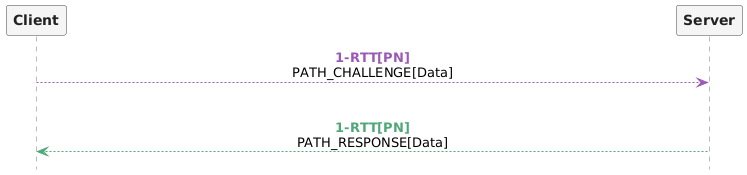
\includegraphics[width=0.7\linewidth]{fig/QUIC/quic_path_validation.png}
        \caption{Diagrama de tempo da validação de caminhos com o QUIC.}
        \label{fig:quic_path_validation}
\end{figure}

Esse processo se assemelha às verificações de conectividade do ICE (Seção~\ref{sec:ice}). O RFC~9000, no entanto, afirma que a validação de caminho não foi projetada como mecanismo de travessia de NAT. Ainda assim, a semelhança motivou propostas como a de \citep{draft-seemann-quic-nat-traversal}, que estende a validação de caminho, inclusive permitindo que o servidor a inicie, com o objetivo de viabilizar o \textit{hole punching} diretamente sobre o QUIC.

\subsubsection{Funcionamento da migração de conexão}
\label{sec:quic_connection_migration_process}

Para migrar, o \textit{endpoint} precisa dispor de um \textit{Connection ID} ainda não utilizado, fornecido pelo outro \textit{endpoint} (Seção~\ref{sec:connection_ids_operation}), que passa a ser usado como DCID no novo caminho. Essa troca impede que um observador correlacione os pacotes enviados antes e depois da migração. Se o outro \textit{endpoint} utilizar \textit{Connection IDs} de tamanho zero, a conexão fica associada ao endereço e à porta, e o tráfego nos dois caminhos se torna correlacionável; por isso, o \textit{endpoint} não deve iniciar a migração nesse caso.

Os pacotes trocados durante uma migração classificam-se em \textit{probing} e \textit{non-probing} \citep{rfc9000}. Um pacote \textit{probing} contém apenas \textit{frames} \texttt{PATH\_\allowbreak{}CHALLENGE}, \texttt{PATH\_\allowbreak{}RESPONSE}, \texttt{NEW\_\allowbreak{}CONNECTION\_\allowbreak{}ID} e \texttt{PADDING}, e serve para sondar um caminho sem migrar a conexão. Qualquer outro pacote é \textit{non-probing}; quando o servidor recebe, a partir de um novo endereço, um pacote \textit{non-probing} com o maior número de pacote já recebido, ele passa a utilizar esse endereço como destino, o que efetiva a migração.

Este trabalho distingue dois tipos de migração, denominação que não consta do RFC~9000. Na migração intencional, o cliente valida previamente o novo caminho com pacotes \textit{probing} e, em seguida, passa a enviar pacotes \textit{non-probing} por ele; o cliente pode também validar um caminho apenas para utilizá-lo posteriormente. Na migração não intencional, o endereço do cliente muda sem que ele o perceba, como em um \textit{NAT rebinding}, no qual o NAT altera o mapeamento de endereço ou de porta associado ao cliente, em geral após um período de inatividade. Nesse caso, o servidor recebe pacotes \textit{non-probing} de um novo endereço, passa a enviar pacotes a esse endereço, sujeito ao limite de amplificação, e inicia a validação do novo caminho. As Figuras~\ref{fig:quic_intentional_migration} e~\ref{fig:quic_non_intentional_migration} ilustram os dois casos.

\begin{figure}[ht]
    \centering
    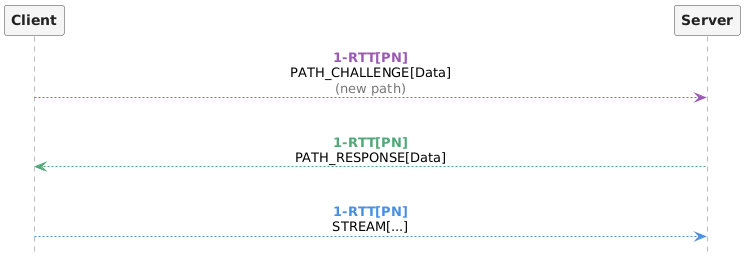
\includegraphics[width=0.6\textwidth]{fig/QUIC/quic_intentional_connection_migration.png}
    \caption{Diagrama de tempo da migração de conexão intencional.}
    \label{fig:quic_intentional_migration}
\end{figure}

\begin{figure}[ht]
    \centering
    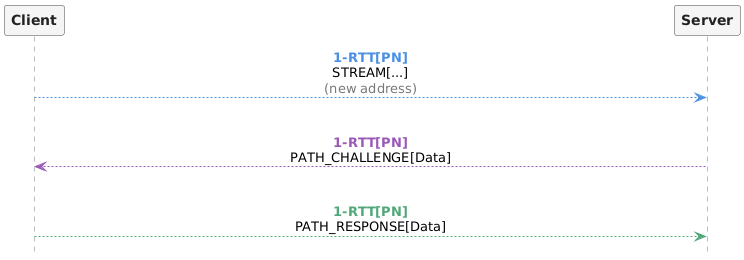
\includegraphics[width=0.6\textwidth]{fig/QUIC/quic_non_intentional_connection_migration.png}
    \caption{Diagrama de tempo da migração de conexão não intencional.}
    \label{fig:quic_non_intentional_migration}
\end{figure}

\section{QUIC Hole Punching}
\label{sec:quic_hole_punching}

O QUIC possui propriedades que favorecem técnicas de travessia de NAT. Por operar sobre UDP, beneficia-se do comportamento dos NATs que torna o \textit{hole punching} UDP mais eficaz que o TCP (Seção~\ref{sec:udp_hole_punching}). Além disso, a validação de caminho e a migração de conexão, embora não tenham sido projetadas para esse fim, podem apoiar essas técnicas (Seção~\ref{sec:quic_path_validation}).

Entre as propostas existentes, \citep{draft-seemann-quic-nat-traversal} apresenta duas formas de travessia de NAT com o QUIC.

A primeira utiliza o ICE (Seção~\ref{sec:ice}) sem alterações no QUIC e exige apenas que pacotes QUIC e STUN possam ser demultiplexados na mesma porta. Os \textit{peers} coletam seus candidatos ICE, trocam-nos por meio de um servidor de sinalização e executam as verificações de conectividade do ICE (Seção~\ref{sec:ice_connectivity_checks}). Concluído o \textit{hole punching}, os \textit{peers} estabelecem a conexão QUIC pelo par de candidatos selecionado.

A segunda abordagem integra a travessia de NAT ao próprio QUIC, com modificações em \textit{frames} e no processo de validação de caminho (Seção~\ref{sec:quic_path_validation}). Nessa abordagem, cliente e servidor estabelecem inicialmente uma conexão por meio de um terceiro servidor com endereço público, como um \textit{relay} ou \textit{proxy}. O cliente obtém seus candidatos de endereço, e o servidor anuncia os seus ao cliente por meio de um novo tipo de \textit{frame}. O cliente define a ordem de teste dos candidatos e sinaliza ao servidor o início do \textit{hole punching}; ambos iniciam então, simultaneamente, a validação de caminho para o mesmo par de candidatos, o que abre os mapeamentos nos NATs de ambos os lados. Trabalhos como \citep{draft-bruynooghe-n0-quic-nat-traversal} estendem essa abordagem com técnicas como o QUIC \textit{multipath} \citep{draft-quic-multipath-06}.

Essa abordagem exige alterações no protocolo, como três novos tipos de \textit{frame}, e permite que o servidor inicie a validação de caminho, o que o RFC~9000 não admite. O próprio \textit{draft} reconhece que essa extensão expõe a conexão a um risco semelhante ao de ataques de amplificação, sem apresentar uma mitigação completa.

Além dessas propostas, \citep{liang2024nat} compara técnicas de \textit{hole punching} TCP (Seção~\ref{sec:tcp_hole_punching}) e QUIC. Até a escrita deste trabalho, entretanto, o IETF não publicou nenhum RFC sobre travessia de NAT com o QUIC, e questões como o risco de amplificação permanecem em aberto.

\begin{comment}
    
\section{QUIC para Aplicações P2P}

\cgk{verificar se isso não vai pra outro lugar}

\subsection{QUIC para Aplicações P2P real-time}

\subsection{QUIC para Aplicações P2P IoT}

\end{comment}
